\chapter{Diseño del sistema}
\label{ch:diseno}

\paragraph*{}
La etapa de diseño es una fase clave dentro del desarrollo de la aplicación, ya que permite transformar los requisitos definidos anteriormente en una solución técnica concreta \cite{pressman2015}. En este punto el proyecto deja de ser solo una lista de necesidades y empieza a tomar forma: se decide cómo se organiza el sistema, cómo se comunican sus partes y de qué manera el usuario va a interactuar con los resultados.

\paragraph*{}
En este Trabajo Fin de Grado, además, el diseño tiene una particularidad importante. La aplicación no se construye desde cero, sino que parte de un dashboard previo que ya ofrecía funcionalidades de carga de datos, preprocesamiento y análisis de supervivencia. Por tanto, la solución diseñada se plantea como una ampliación ordenada del sistema existente. La idea no es romper la base anterior, sino aprovecharla y hacerla crecer con nuevos modelos, nuevas visualizaciones, soporte multilingüe, exportación de informes e interpretación asistida por inteligencia artificial.

\section{Arquitectura del sistema}

\paragraph*{}
La arquitectura del sistema se organiza siguiendo una estructura modular. Esta decisión resulta bastante natural para una aplicación desarrollada en Python y Dash, ya que permite separar la interfaz, la lógica de análisis, la generación de informes y los servicios auxiliares. Gracias a esta división, cada parte del sistema tiene una responsabilidad concreta y es más sencillo mantener el proyecto, localizar errores o incorporar nuevas técnicas de análisis en el futuro.

\paragraph*{}
Desde un punto de vista general, el sistema puede entenderse como una aplicación web local compuesta por varias capas. En primer lugar, se encuentra la capa de presentación, construida con Dash, HTML y componentes interactivos. Esta capa es la que ve el usuario: menús, formularios, botones, tablas, gráficas y modales de exportación. En segundo lugar, aparece la capa de control, formada principalmente por los callbacks de Dash, que conectan las acciones del usuario con la lógica interna de la aplicación. Por último, se encuentra la capa de procesamiento, donde se ejecutan los modelos estadísticos, las transformaciones de datos, la generación de visualizaciones, la creación de PDFs y las peticiones al módulo de inteligencia artificial.

\paragraph*{}
La separación por capas se completa con una distribución por componentes. En lugar de concentrar toda la lógica en una única parte de la aplicación, el diseño distingue entre navegación, presentación visual, gestión de eventos, preparación de datos, ejecución de modelos, visualización de resultados, generación de informes, traducción de textos e interpretación mediante inteligencia artificial. Esta visión resulta más clara para entender el sistema en conjunto, mientras que los archivos concretos que materializan cada responsabilidad se detallan más adelante en el capítulo de implementación.

\paragraph*{}
Esta organización también facilita la ampliación del dashboard. Si se incorpora una nueva técnica de supervivencia, no es necesario replantear toda la aplicación: basta con integrarla dentro del componente de análisis, conectarla con la interfaz y, si procede, añadir sus visualizaciones y su exportación. La verdad es que esta idea es importante, porque el proyecto parte de un sistema previo y necesita crecer sin perder estabilidad ni coherencia.

\begin{table}[H]
\centering
\small
\begin{tabular}{|p{0.35\textwidth}|p{0.55\textwidth}|}
\hline
\textbf{Componente de diseño} & \textbf{Responsabilidad principal} \\ \hline
Interfaz de usuario & Presenta las pantallas, controles, tablas, gráficas, botones y modales con los que interactúa el usuario. \\ \hline
Gestor de navegación & Organiza el acceso a las distintas secciones del dashboard y mantiene un recorrido coherente entre carga, análisis, comparación y exportación. \\ \hline
Gestor de interacción & Recibe las acciones del usuario y coordina la respuesta del sistema, conectando la interfaz con los procesos internos. \\ \hline
Gestor de datos & Controla la carga, validación, limpieza y preparación del dataset antes de ejecutar los modelos. \\ \hline
Motor de análisis & Agrupa las técnicas estadísticas y predictivas utilizadas para estudiar la supervivencia académica. \\ \hline
Generador de visualizaciones & Transforma los resultados de los modelos en gráficas, curvas, tablas y comparaciones interpretables. \\ \hline
Generador de informes & Prepara la exportación de resultados en documentos reutilizables, incorporando tablas, gráficos e interpretaciones. \\ \hline
Módulo de inteligencia artificial & Produce explicaciones textuales de apoyo a partir de los resultados obtenidos en los análisis. \\ \hline
Sistema de internacionalización & Gestiona los textos de la interfaz y permite adaptar la aplicación a castellano e inglés. \\ \hline
\end{tabular}
\caption{Componentes principales de la arquitectura del sistema}
\label{tab:modulos_sistema}
\end{table}

\section{Diseño de los datos de análisis}

\paragraph*{}La ampliación del sistema se apoya en un conjunto de variables que permiten estudiar el abandono académico desde una perspectiva temporal y, además, relacionarlo con características concretas del estudiante. Algunas de ellas son imprescindibles para cualquier modelo de supervivencia, mientras que otras actúan como covariables y permiten comparar perfiles o alimentar modelos más complejos, como la regresión de Cox, el Test de Log-Rank o Random Survival Forest.

\paragraph*{}La selección de estas variables no se ha realizado de forma arbitraria. Se han priorizado aquellas que cumplen tres criterios principales: que estén disponibles de forma estable en el conjunto de datos, que tengan una interpretación clara dentro del contexto académico y que puedan aportar información útil sobre la permanencia o el abandono del estudiante. También se ha buscado mantener un equilibrio razonable entre riqueza analítica y claridad, ya que incluir demasiadas variables puede hacer que los resultados sean más difíciles de explicar.

\small
\begin{longtable}{|>{\raggedright\arraybackslash}p{3.2cm}|>{\raggedright\arraybackslash}p{4.2cm}|>{\raggedright\arraybackslash}p{6.1cm}|}
\hline
\textbf{Variable o grupo} & \textbf{Qué representa} & \textbf{Motivo de selección} \\ \hline
\endfirsthead

\hline
\textbf{Variable o grupo} & \textbf{Qué representa} & \textbf{Motivo de selección} \\ \hline
\endhead

Identificador del estudiante \newline \texttt{id\_student} & Identifica de forma única a cada estudiante dentro del conjunto de datos. & Se utiliza para consolidar registros y evitar duplicidades durante el preprocesamiento. No es una covariable explicativa, pero resulta necesaria para construir un dataset limpio y coherente. \\ \hline

Tiempo observado \newline \texttt{date} & Indica el tiempo de seguimiento utilizado por los modelos de supervivencia. & Es una variable imprescindible, ya que el objetivo del análisis no es solo saber si se produce el abandono, sino estudiar cuándo ocurre. \\ \hline

Evento de abandono \newline \texttt{final\_result} & Recoge el resultado final del estudiante y permite identificar si se produce el evento de abandono. & Es la variable que define el evento analizado. Se transforma en una variable binaria para diferenciar abandono y no abandono dentro de los modelos. \\ \hline

Género \newline \texttt{gender\_F} & Representa el género del estudiante mediante una codificación binaria. & Se incluye porque permite analizar si existen diferencias de permanencia entre grupos. Además, es una variable sencilla de interpretar y útil para segmentar resultados. \\ \hline

Discapacidad \newline \texttt{disability\_N} & Indica si el estudiante aparece registrado con o sin discapacidad. & Se selecciona por su relevancia en el contexto educativo, ya que puede estar relacionada con necesidades de apoyo, accesibilidad o condiciones que influyen en la trayectoria académica. \\ \hline

Tramo de edad \newline \texttt{age\_band} & Agrupa al alumnado en rangos de edad: \texttt{0-35}, \texttt{35-55} y \texttt{55<=}. & Se incluye porque la edad puede reflejar perfiles académicos distintos: estudiantes jóvenes, personas que retoman estudios o alumnado con otras responsabilidades. Esto permite comparar curvas y riesgos entre grupos. \\ \hline

Nivel educativo previo \newline \texttt{highest\_education} & Describe la formación máxima alcanzada antes de acceder al curso o programa analizado. & Se considera relevante porque la preparación académica previa puede influir en la adaptación al entorno universitario y, por tanto, en la probabilidad de permanencia o abandono. \\ \hline

Créditos estudiados \newline \texttt{studied\_credits} & Refleja la carga académica asumida por el estudiante. & Se incorpora porque permite estudiar si la dedicación académica o el volumen de créditos se relaciona con el abandono. Además, es una variable no binaria, por lo que ayuda a cumplir el objetivo de ampliar el análisis más allá de variables simples. \\ \hline

\caption{Variables principales utilizadas y justificación de su selección}
\label{tab:variables_analisis}\\
\end{longtable}
\normalsize

\paragraph*{}Aunque el conjunto de datos puede contener más atributos procedentes del sistema original, como actividad en recursos, módulos, presentaciones, regiones o intentos previos, esta ampliación se centra especialmente en las variables anteriores. La razón es que permiten cubrir los objetivos del trabajo sin perder claridad: se conserva la información mínima necesaria para los modelos de supervivencia y se incorporan covariables personales y académicas que enriquecen la interpretación de los resultados. Otras variables podrían ser útiles en futuros análisis, pero en esta versión se ha optado por un conjunto más controlado, comprensible y directamente relacionado con los casos de uso definidos.

\section{Diseño de la interfaz}

\paragraph*{}
El diseño de la interfaz mantiene la idea principal del dashboard original: ofrecer al usuario un entorno visual desde el que pueda cargar datos, ejecutar análisis y consultar resultados sin tener que trabajar directamente con código. La verdad es que este punto es importante, porque el sistema está pensado para facilitar el análisis de supervivencia en un contexto académico, donde no siempre se parte de un perfil técnico avanzado.

\paragraph*{}
La navegación se estructura mediante diferentes páginas o secciones. Cada una agrupa funcionalidades relacionadas: carga y visualización del dataset, análisis de covariables, técnicas de supervivencia, comparación de modelos y exportación de resultados. Esta organización evita mezclar demasiada información en una sola pantalla y permite que el usuario avance poco a poco, como si siguiera un pequeño recorrido: primero carga los datos, después los prepara, luego ejecuta modelos y finalmente interpreta o exporta los resultados.

\paragraph*{}
Para que ese recorrido se entienda de un vistazo, se ha incorporado un diagrama de navegación de la aplicación. La verdad es que este tipo de esquema ayuda bastante, porque funciona casi como un mapa antes de empezar una ruta: permite ver desde dónde parte el usuario, qué pantallas puede visitar y cómo se conectan las distintas acciones del dashboard. En él se representa el paso desde la carga inicial del dataset hasta la visualización de datos, el análisis de covariables, las técnicas de supervivencia, la comparación de métodos, la interpretación mediante IA y la exportación de resultados.

\begin{figure}[H]
    \centering
    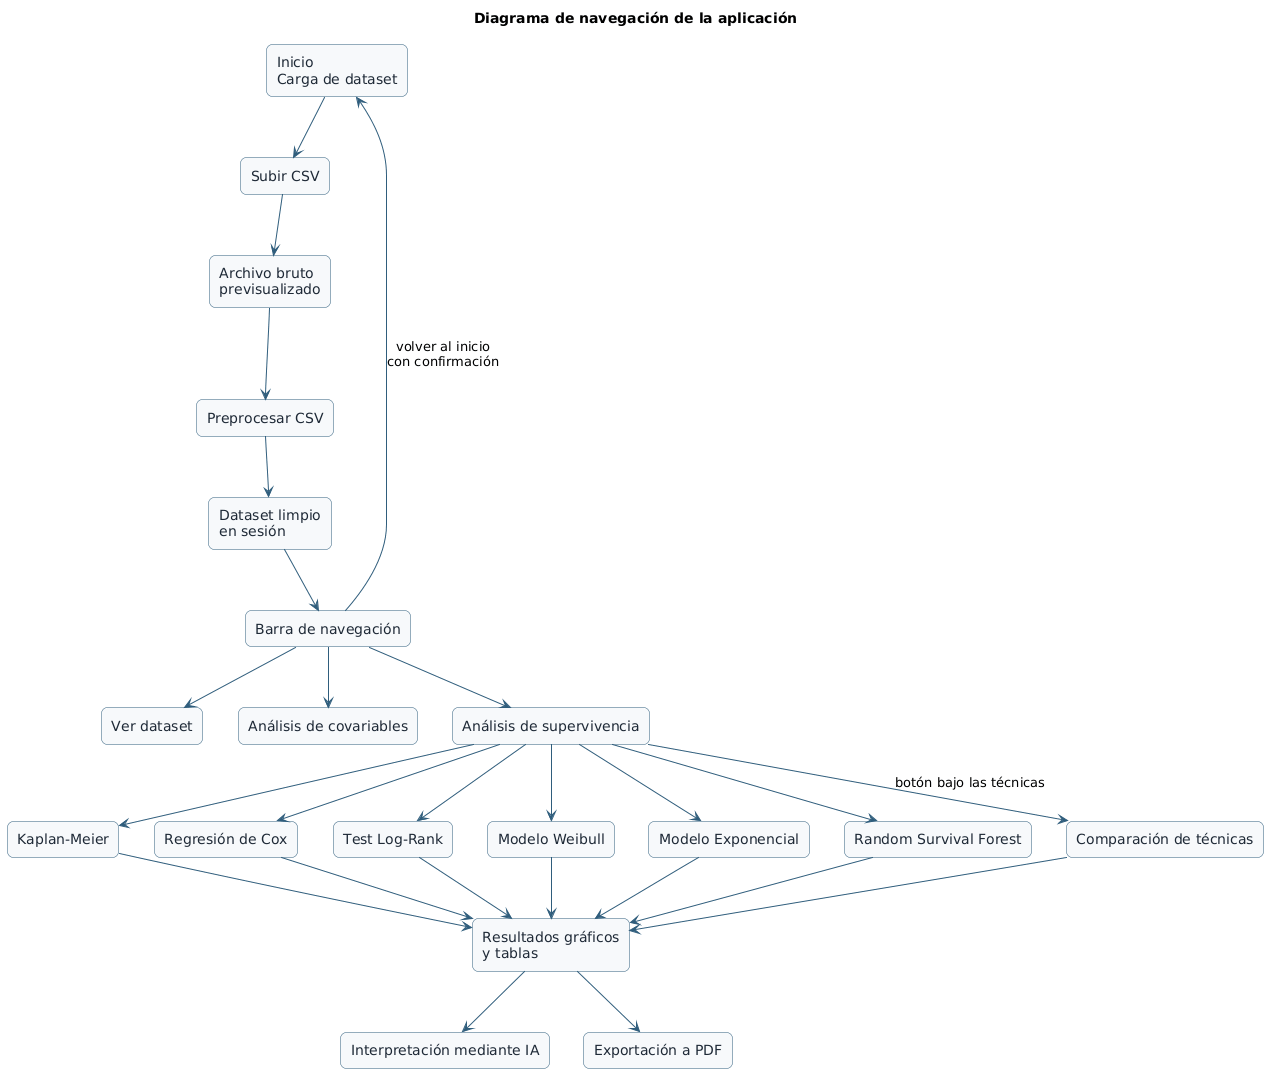
\includegraphics[width=\textwidth]{Imagenes/navegaciion.png}
    \caption{Diagrama de navegación de la aplicación}
    \label{fig:diagrama_navegacion}
\end{figure}

\paragraph*{}
En las páginas de análisis se ha seguido un patrón común. Primero se presenta la técnica seleccionada, después se muestran los controles necesarios y, finalmente, se generan tablas, métricas, gráficas e interpretaciones. Este patrón se repite en modelos como Exponencial, Weibull y Random Survival Forest, lo que aporta coherencia al uso de la aplicación. Cuando el usuario aprende cómo funciona una sección, puede moverse por las demás con menos esfuerzo.

\paragraph*{}
También se ha cuidado el diseño de los modales de exportación. Estos permiten seleccionar qué contenido se desea incluir en el informe, como tablas, gráficos o explicaciones generadas por IA. De esta forma, la exportación no se limita a descargar una captura rígida de la pantalla, sino que ofrece cierto control sobre el resultado final. Además, la interfaz incorpora soporte multilingüe, permitiendo alternar entre castellano e inglés y adaptando los textos visibles de la aplicación al idioma seleccionado.

\subsection{Interfaz de usuario (UI)}

\paragraph*{}
A continuación se muestran las principales pantallas de la interfaz desarrollada. Estas capturas permiten ver el recorrido básico que sigue el usuario dentro del dashboard: desde la entrada inicial al sistema, pasando por la carga y limpieza del archivo de datos, hasta llegar a las secciones de análisis de covariables y análisis de supervivencia.

\begin{figure}[H]
    \centering
    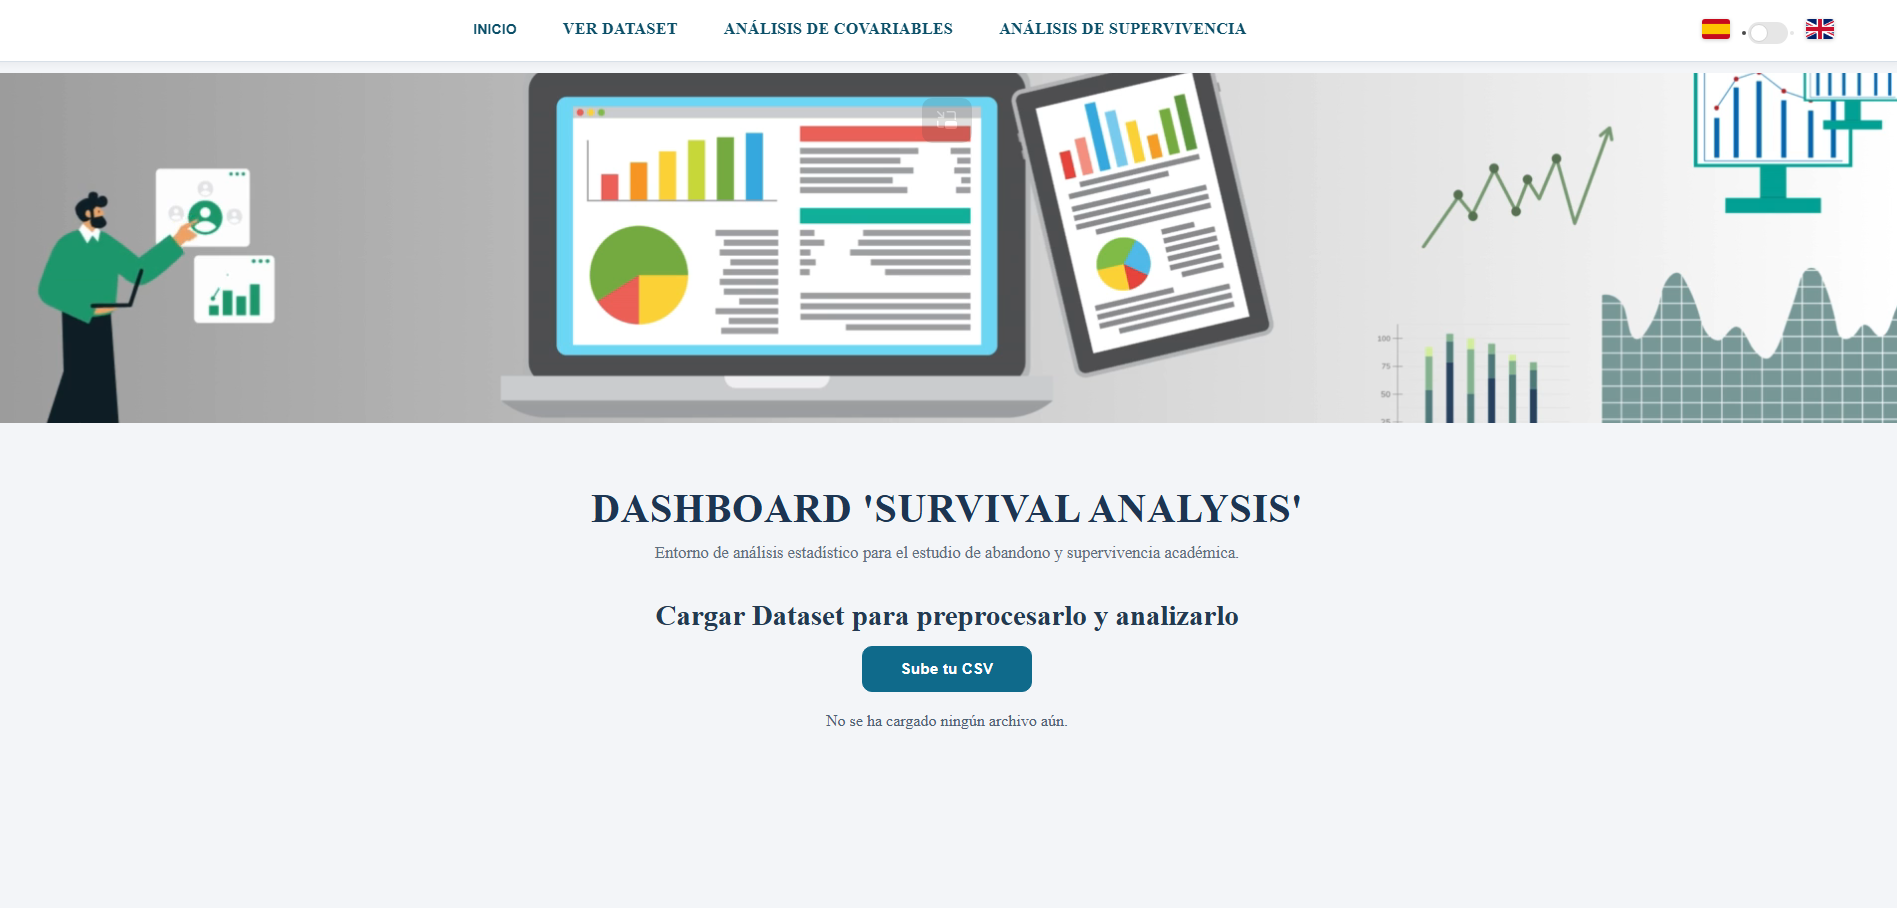
\includegraphics[width=\textwidth]{Imagenes/home.png}
    \caption{Pantalla principal del dashboard}
    \label{fig:interfaz_home}
\end{figure}

\begin{figure}[H]
    \centering
    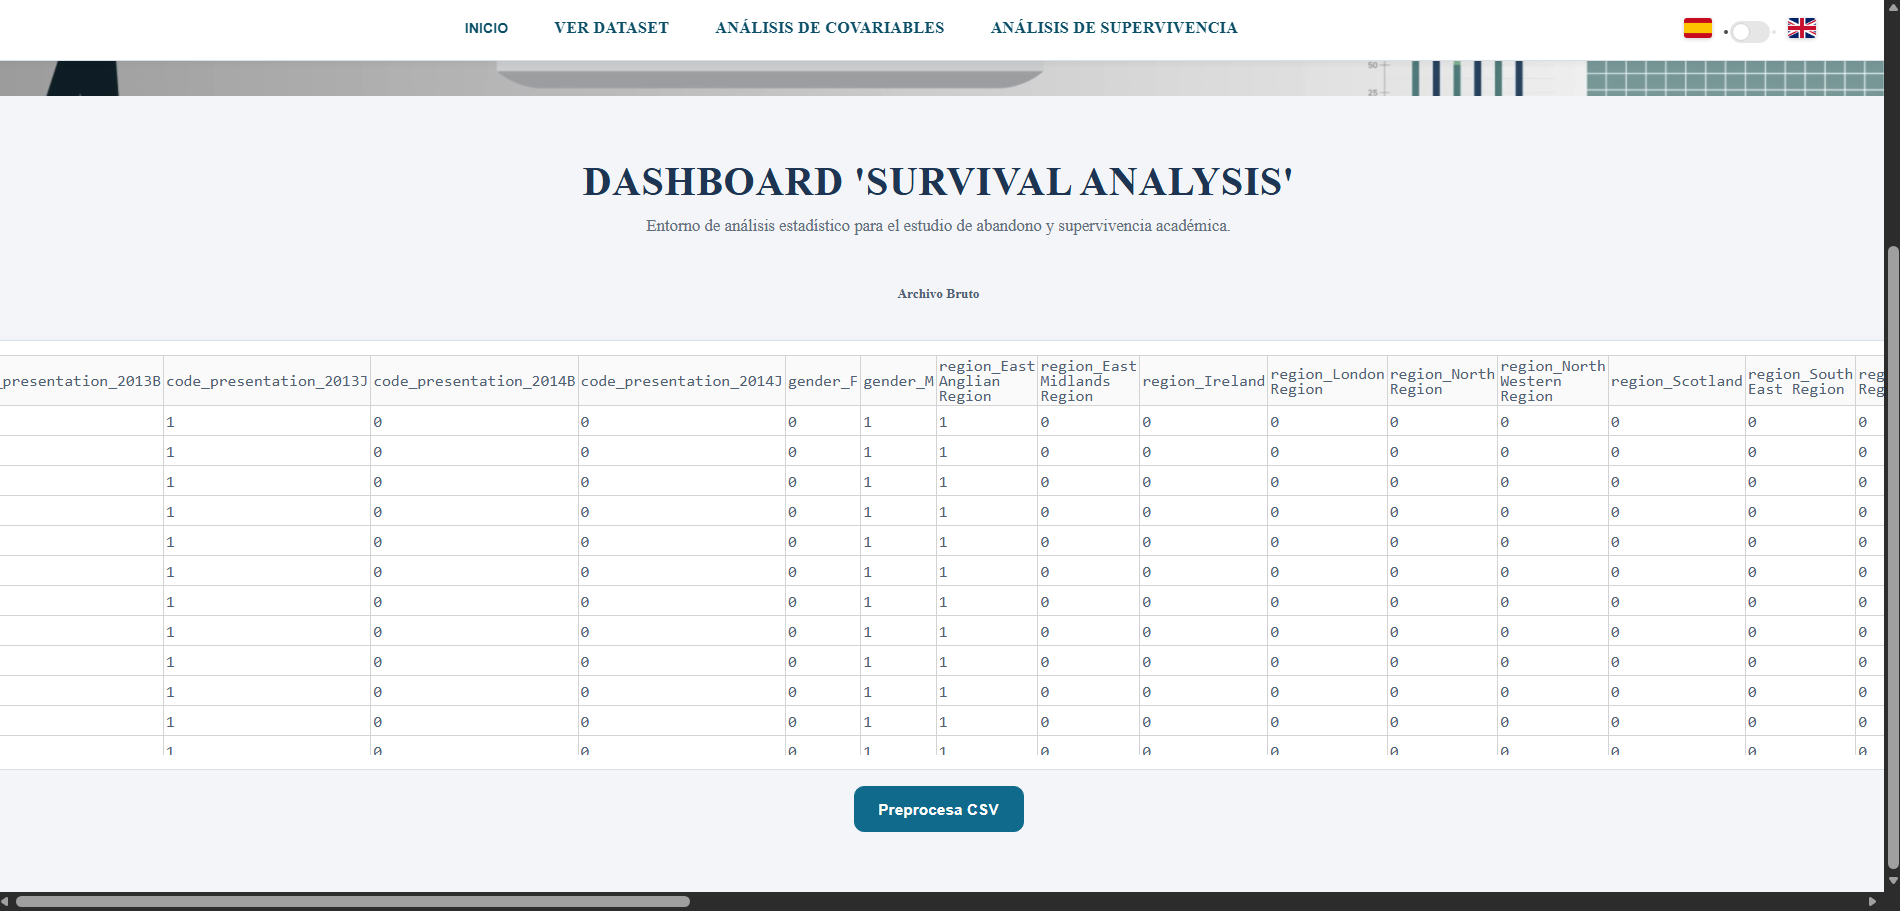
\includegraphics[width=\textwidth]{Imagenes/archivo_bruto.png}
    \caption{Visualización del archivo bruto cargado en el sistema}
    \label{fig:interfaz_archivo_bruto}
\end{figure}

\begin{figure}[H]
    \centering
    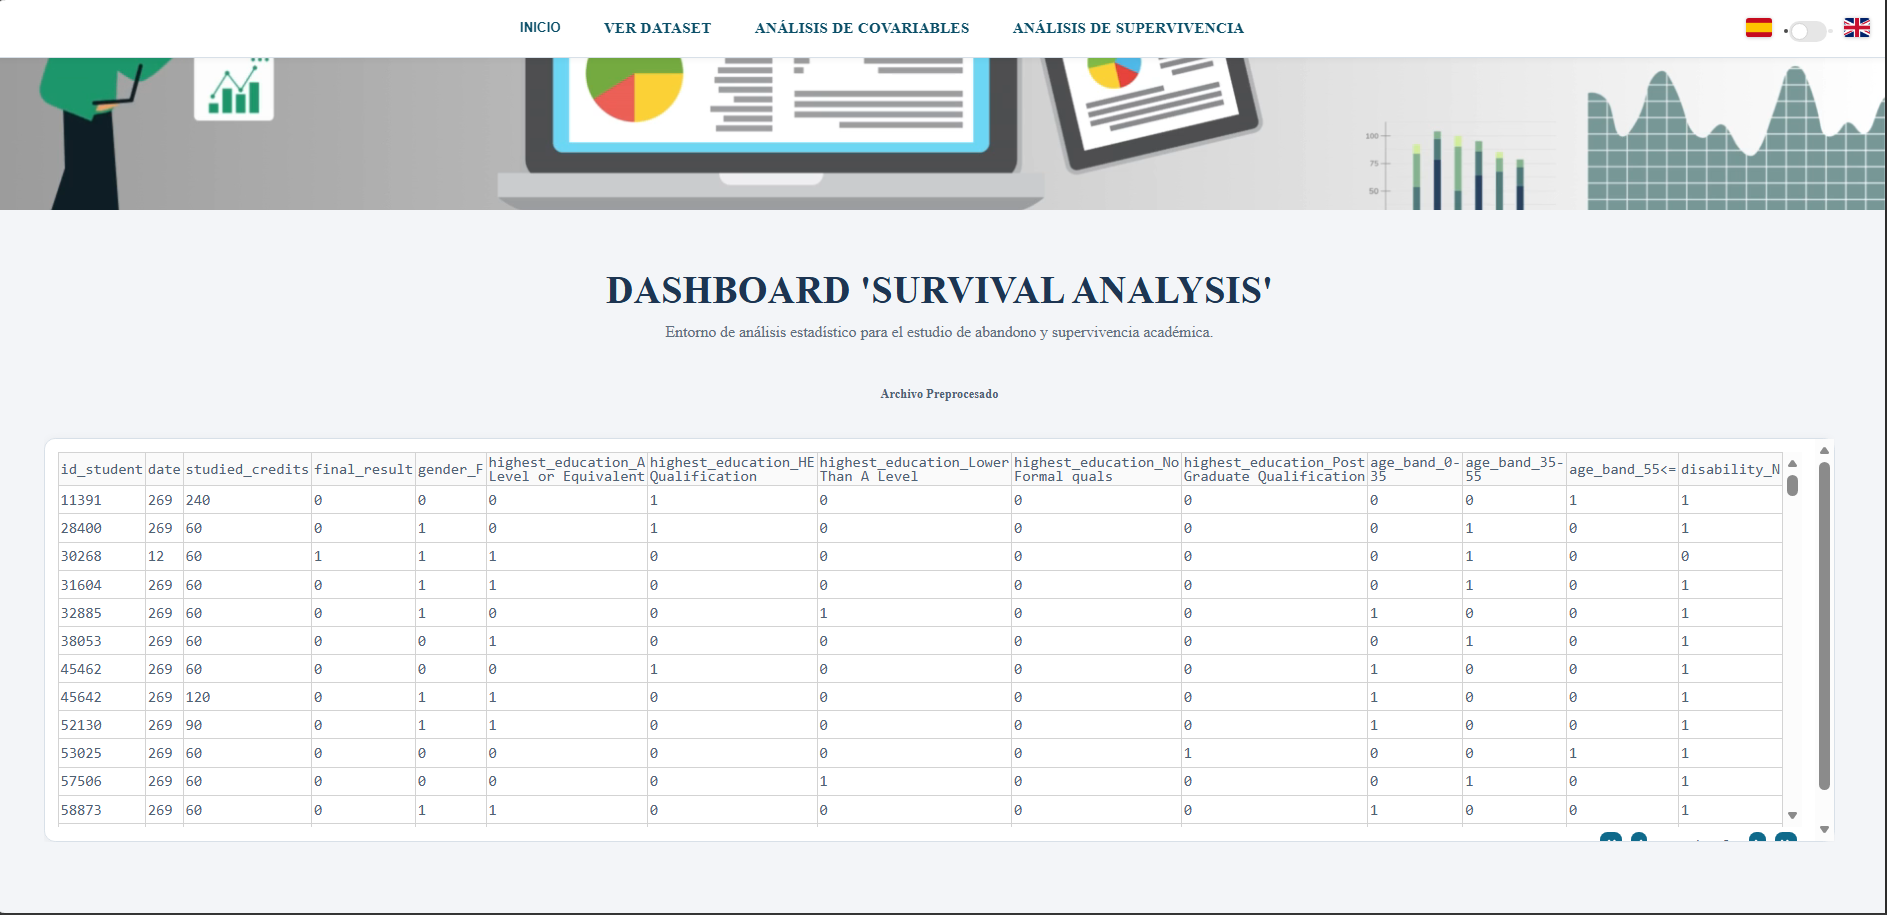
\includegraphics[width=\textwidth]{Imagenes/archivo_limpio.png}
    \caption{Visualización del archivo limpio tras el preprocesamiento}
    \label{fig:interfaz_archivo_limpio}
\end{figure}

\subsubsection*{\underline{Ver dataset}}

\paragraph*{}
La sección de visualización del dataset permite revisar los datos cargados antes y después del proceso de limpieza. Esta parte resulta útil para que el usuario pueda comprobar, de un vistazo, qué información se está utilizando realmente en los análisis posteriores.

\begin{figure}[H]
    \centering
    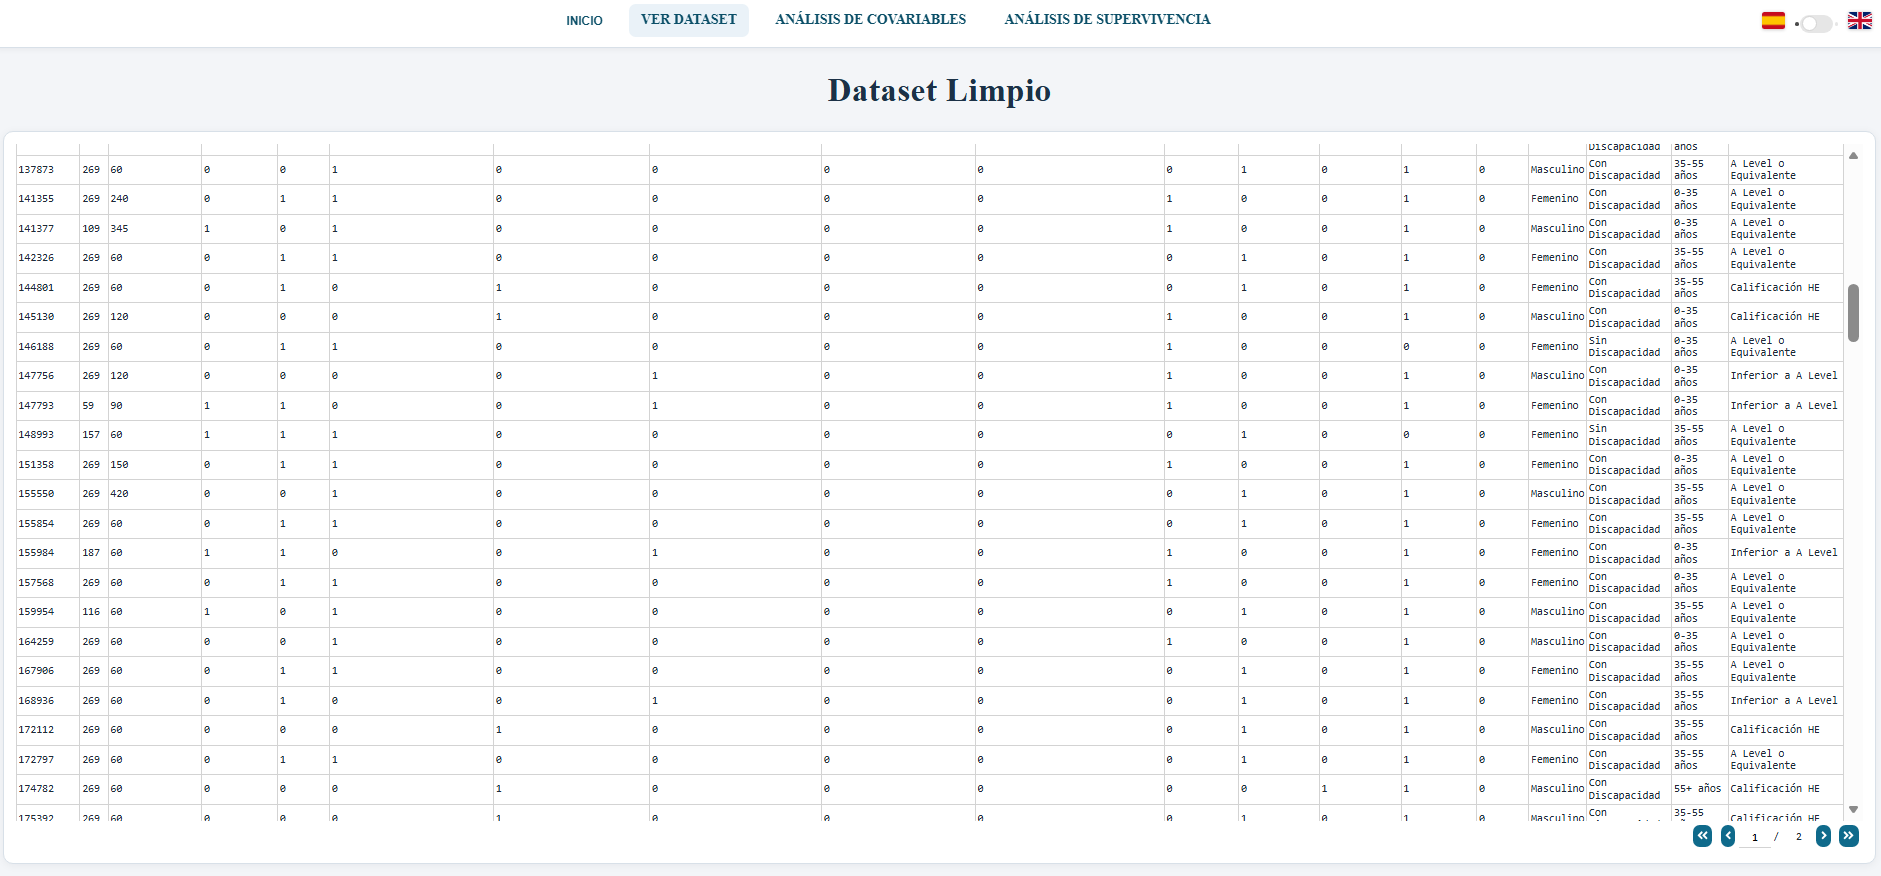
\includegraphics[width=\textwidth]{Imagenes/ver1.png}
    \caption{Vista inicial de la sección Ver dataset}
    \label{fig:interfaz_ver_dataset_1}
\end{figure}

\begin{figure}[H]
    \centering
    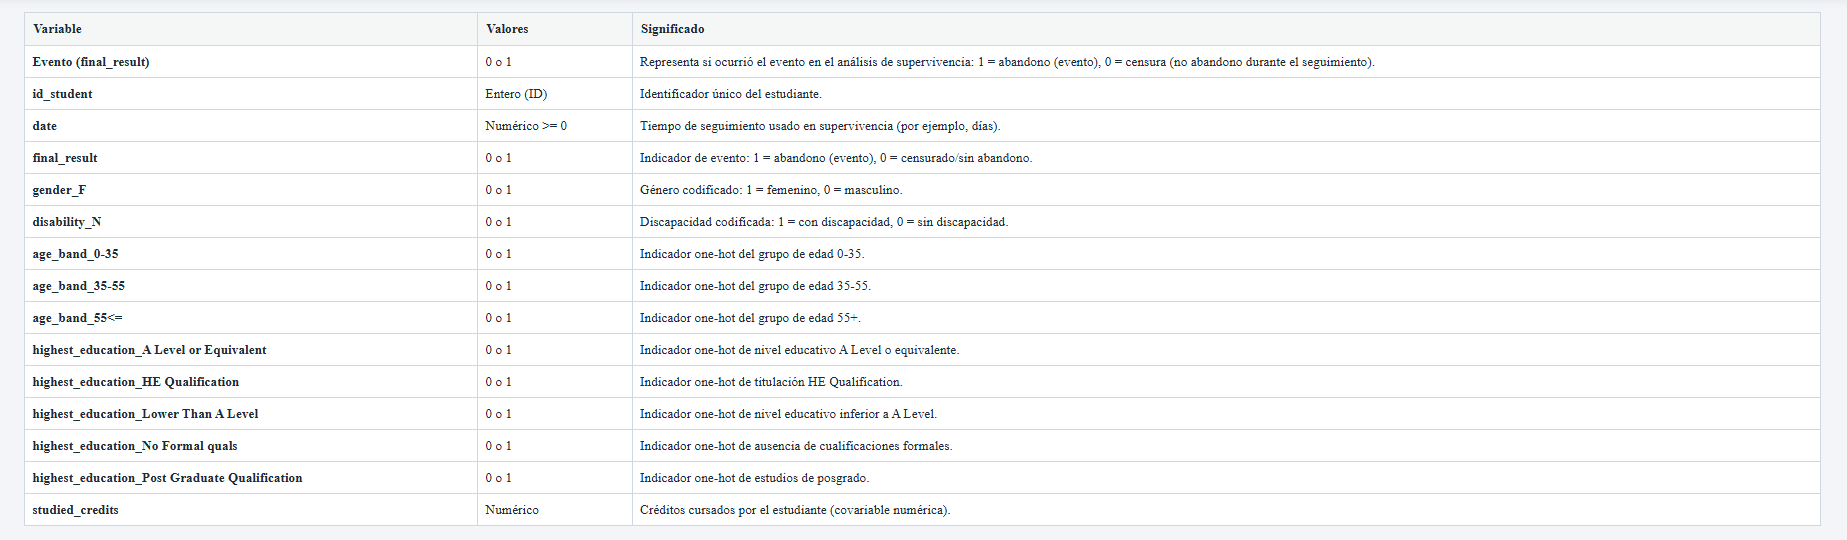
\includegraphics[width=\textwidth]{Imagenes/ver2.png}
    \caption{Detalle de la visualización del dataset dentro del dashboard}
    \label{fig:interfaz_ver_dataset_2}
\end{figure}

\subsubsection*{\underline{Análisis de covariables}}

\paragraph*{}
El análisis de covariables permite explorar la relación entre las variables disponibles y el evento de interés. Esta pantalla sirve como apoyo previo al análisis de supervivencia, ya que ayuda a detectar qué variables pueden aportar información relevante antes de aplicar los modelos estadísticos.

\begin{figure}[H]
    \centering
    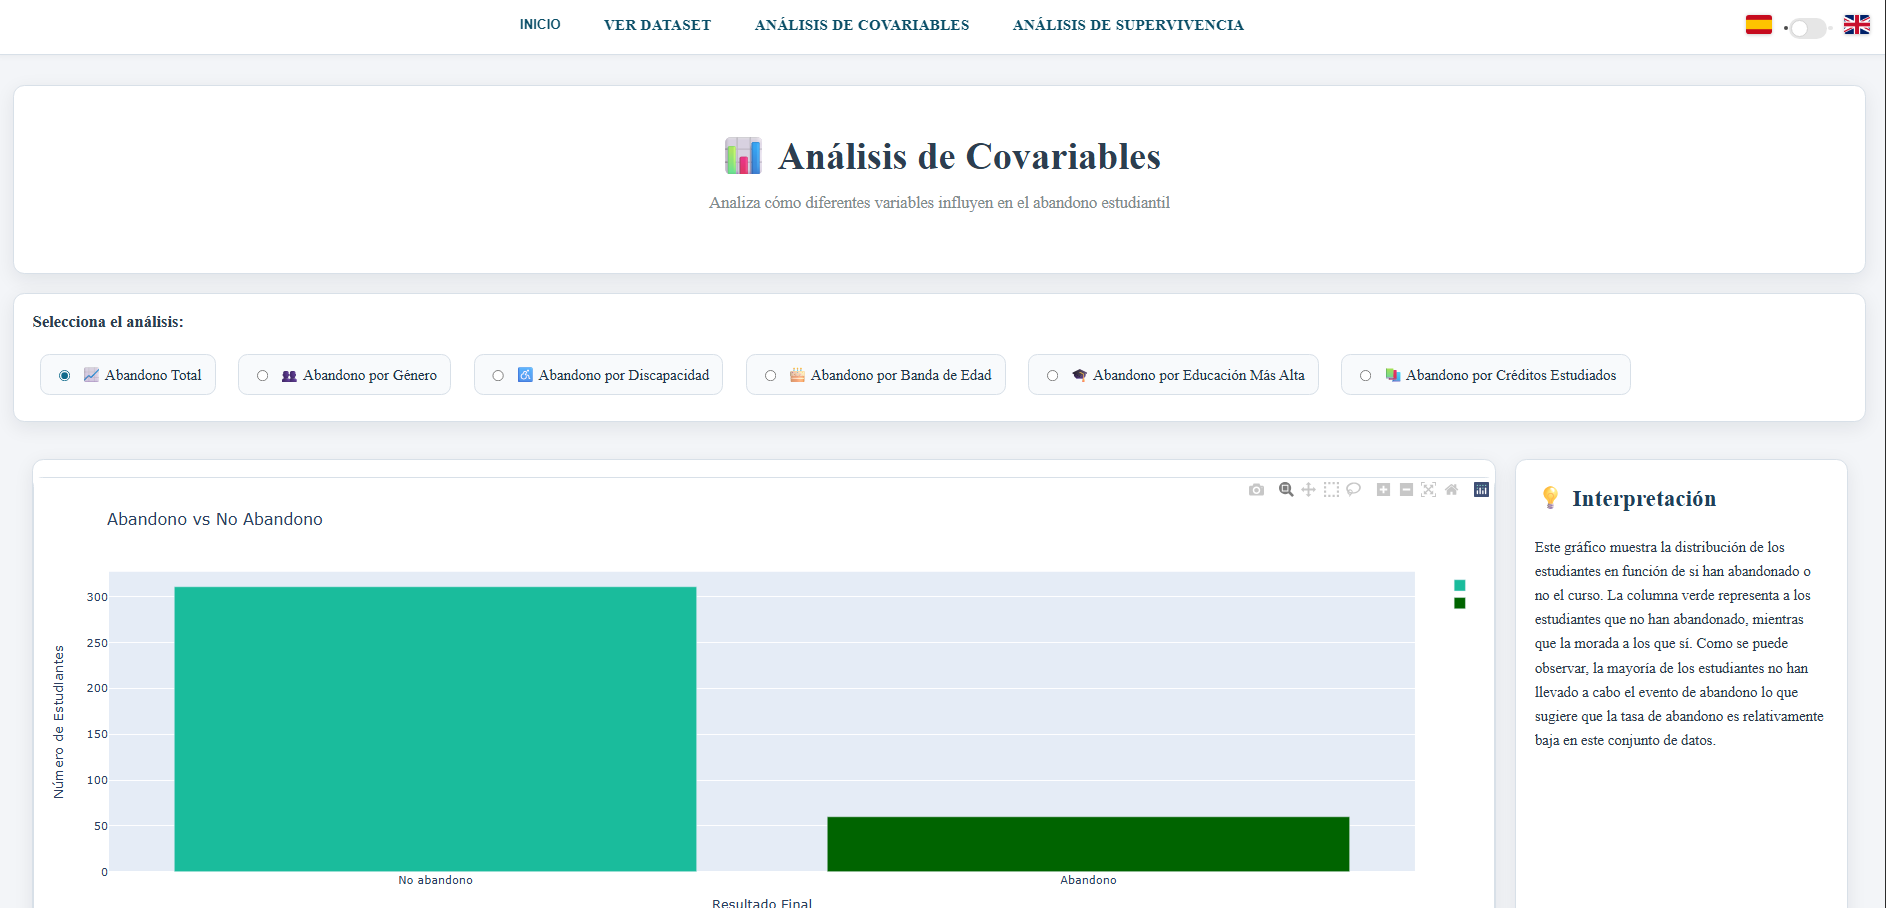
\includegraphics[width=\textwidth]{Imagenes/analisis_covariables.png}
    \caption{Sección de análisis de covariables}
    \label{fig:interfaz_analisis_covariables}
\end{figure}

\subsubsection*{\underline{Análisis de supervivencia}}

\paragraph*{}
La sección de análisis de supervivencia actúa como punto de entrada a las distintas técnicas disponibles en el sistema. Desde esta pantalla el usuario puede acceder a los métodos clásicos, a las nuevas técnicas incorporadas y a la comparación general entre métodos mediante un botón ancho situado bajo el conjunto de técnicas. De este modo, la navegación se mantiene centralizada y fácil de seguir.

\begin{figure}[H]
    \centering
    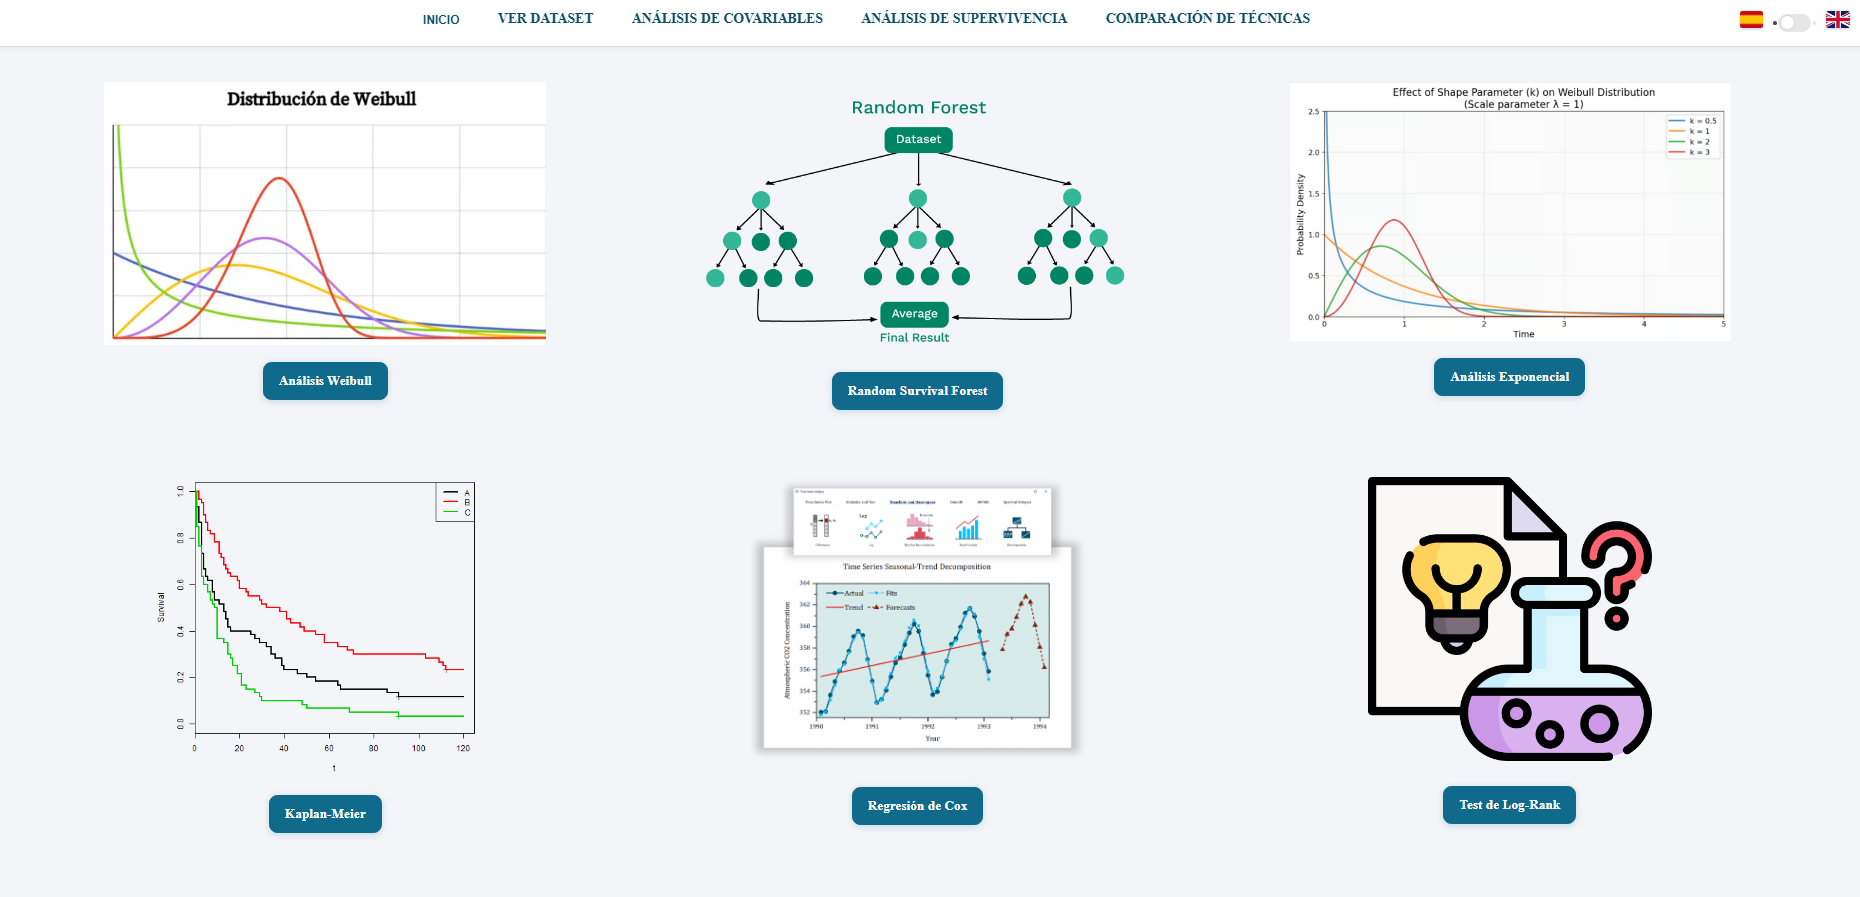
\includegraphics[width=\textwidth]{Imagenes/analisis_superv.png}
    \caption{Sección de análisis de supervivencia}
    \label{fig:interfaz_analisis_supervivencia}
\end{figure}

\subsubsection*{\underline{Kaplan-Meier}}

\paragraph*{}
Dentro del análisis de supervivencia, la sección de Kaplan-Meier permite consultar la curva de supervivencia general, aplicar filtros sobre los datos y exportar los resultados obtenidos. Es una de las vistas más importantes del sistema, ya que ofrece una primera lectura visual de la evolución de la supervivencia en el conjunto de datos.

\begin{figure}[H]
    \centering
    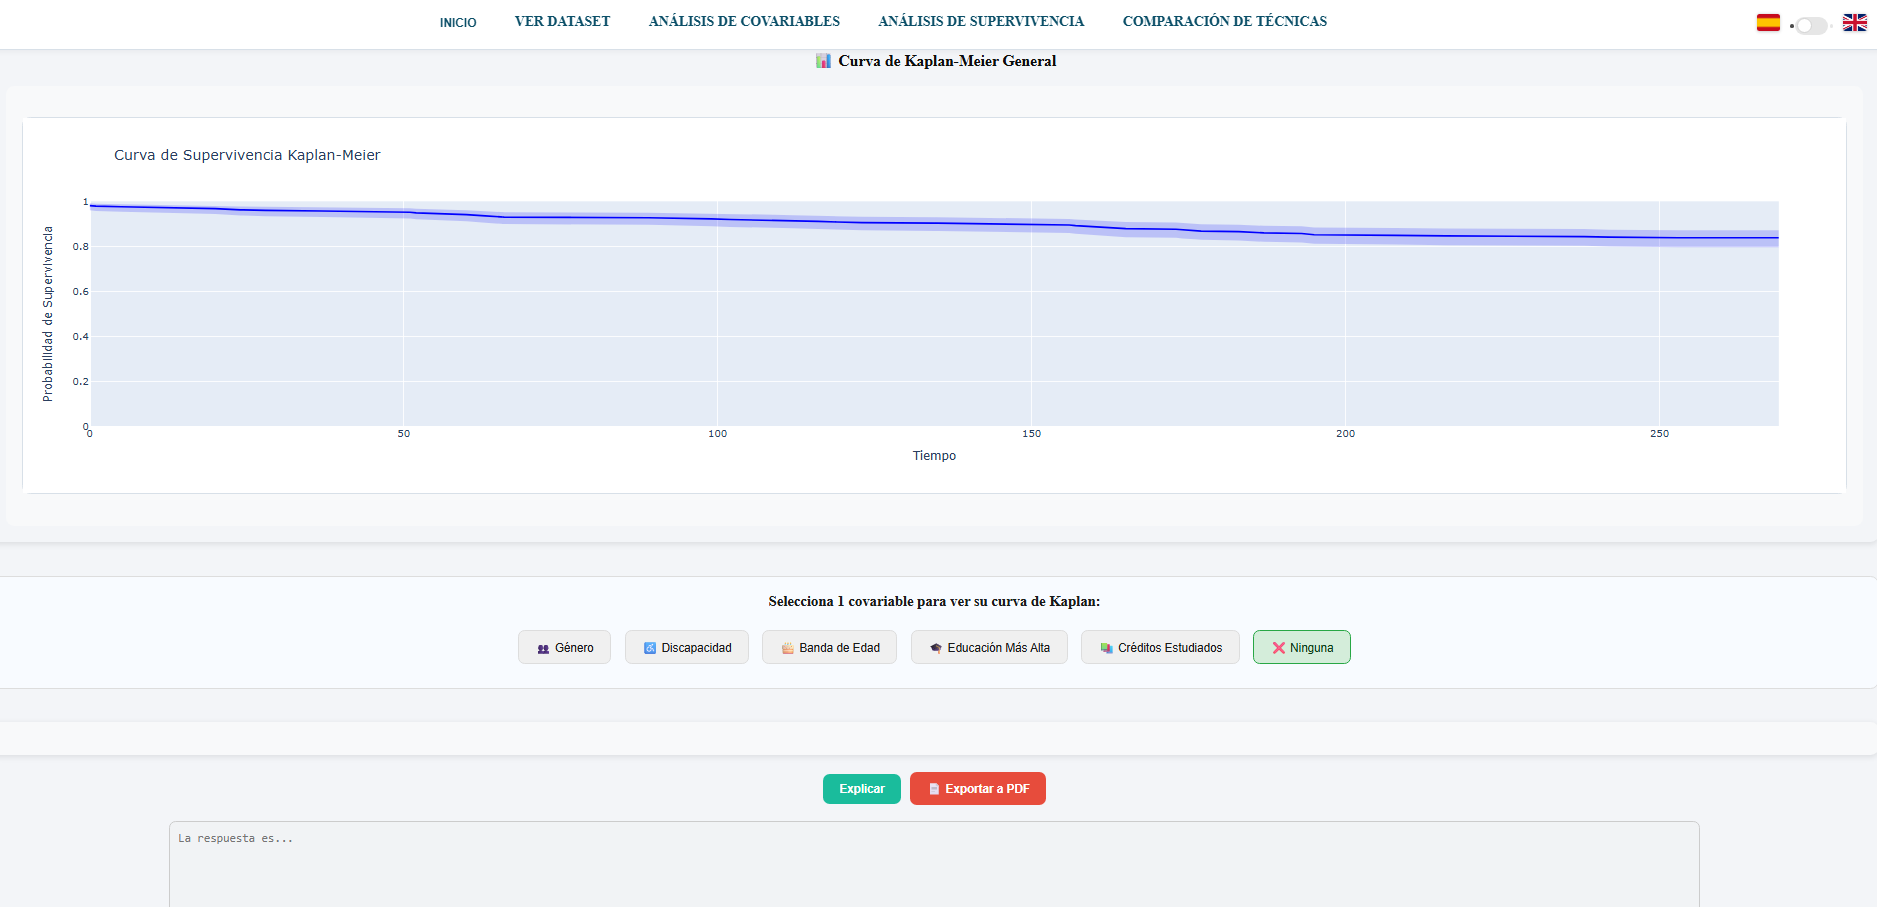
\includegraphics[width=\textwidth]{Imagenes/kp_general.png}
    \caption{Vista general del análisis Kaplan-Meier}
    \label{fig:interfaz_kp_general}
\end{figure}

\begin{figure}[H]
    \centering
    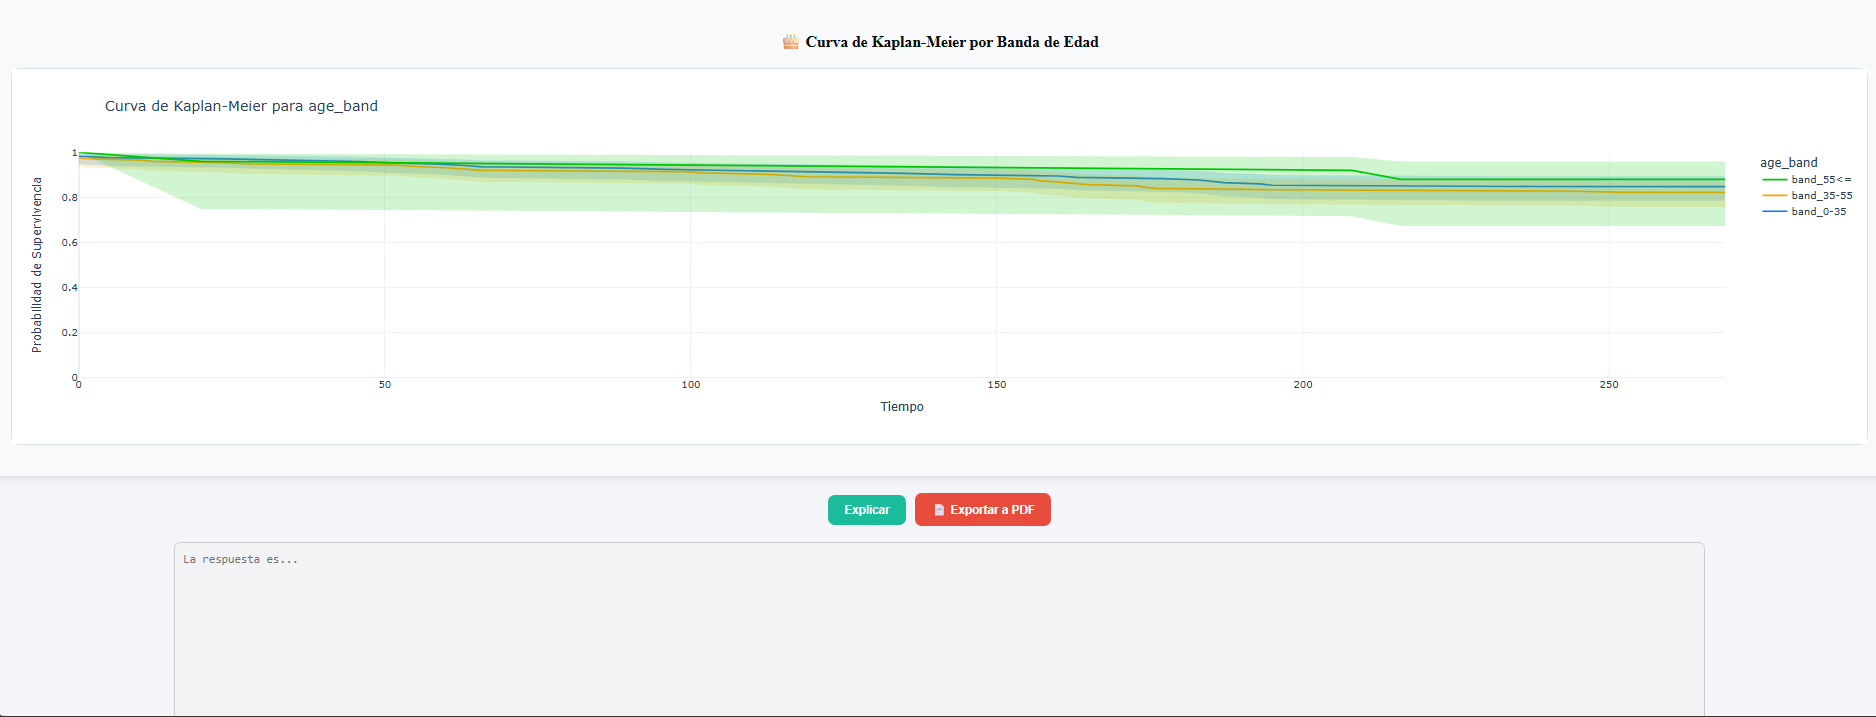
\includegraphics[width=\textwidth]{Imagenes/curva_kp.png}
    \caption{Curva de supervivencia generada mediante Kaplan-Meier}
    \label{fig:interfaz_curva_kp}
\end{figure}

\begin{figure}[H]
    \centering
    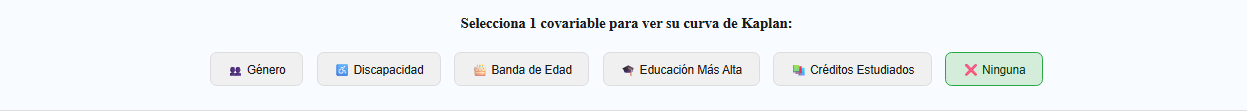
\includegraphics[width=\textwidth]{Imagenes/filtros_kp.png}
    \caption{Filtros disponibles en el análisis Kaplan-Meier}
    \label{fig:interfaz_filtros_kp}
\end{figure}

\begin{figure}[H]
    \centering
    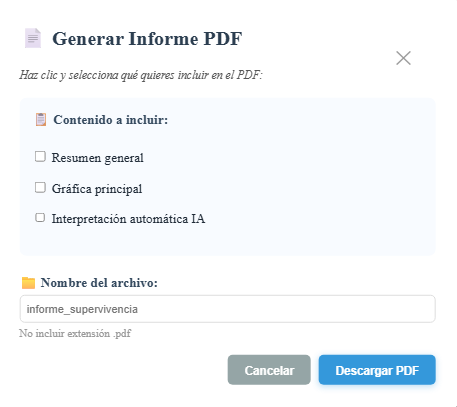
\includegraphics[width=\textwidth]{Imagenes/exportarPDFKp.png}
    \caption{Exportación a PDF de los resultados de Kaplan-Meier}
    \label{fig:interfaz_exportar_pdf_kp}
\end{figure}

\subsubsection*{\underline{Regresión de Cox}}

\paragraph*{}
La vista de regresión de Cox permite analizar la influencia de distintas covariables sobre el tiempo hasta el evento. Además de mostrar los resultados del modelo, la interfaz incorpora filtros, gráficas asociadas y la opción de exportar la información generada.

\begin{figure}[H]
    \centering
    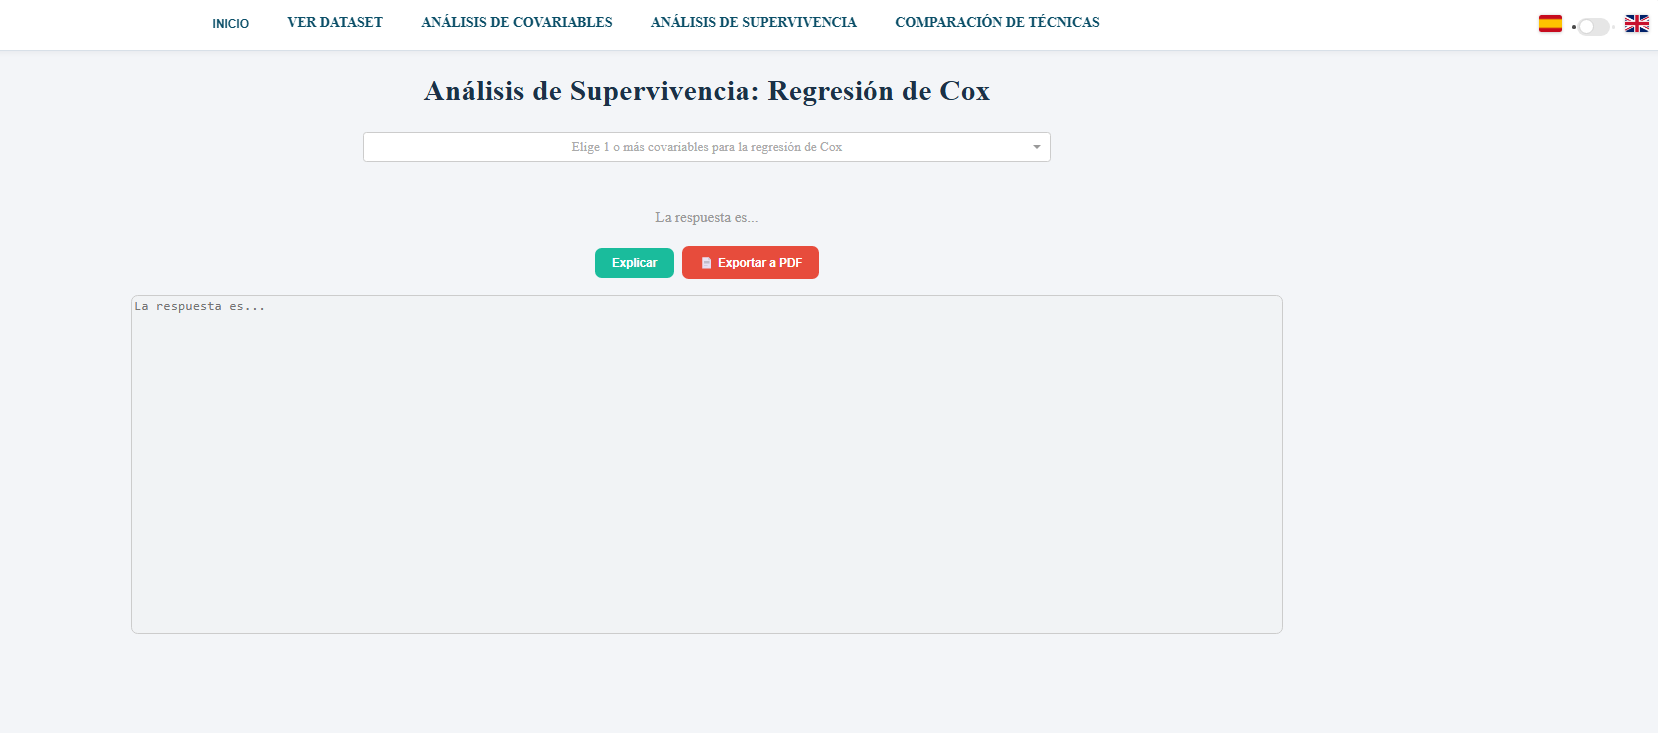
\includegraphics[width=\textwidth]{Imagenes/regresionCox.png}
    \caption{Vista principal de la regresión de Cox}
    \label{fig:interfaz_regresion_cox}
\end{figure}

\begin{figure}[H]
    \centering
    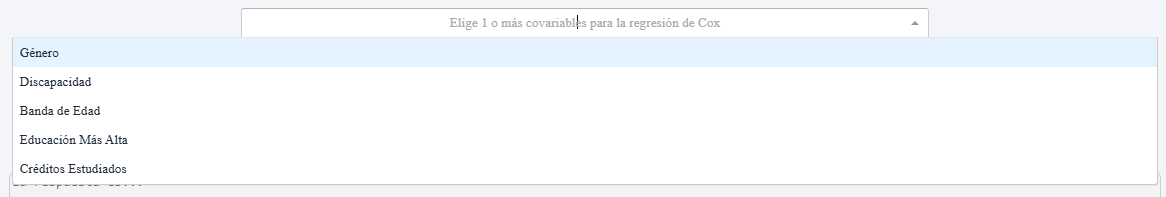
\includegraphics[width=\textwidth]{Imagenes/filtrosCox.png}
    \caption{Filtros utilizados en la regresión de Cox}
    \label{fig:interfaz_filtros_cox}
\end{figure}

\begin{figure}[H]
    \centering
    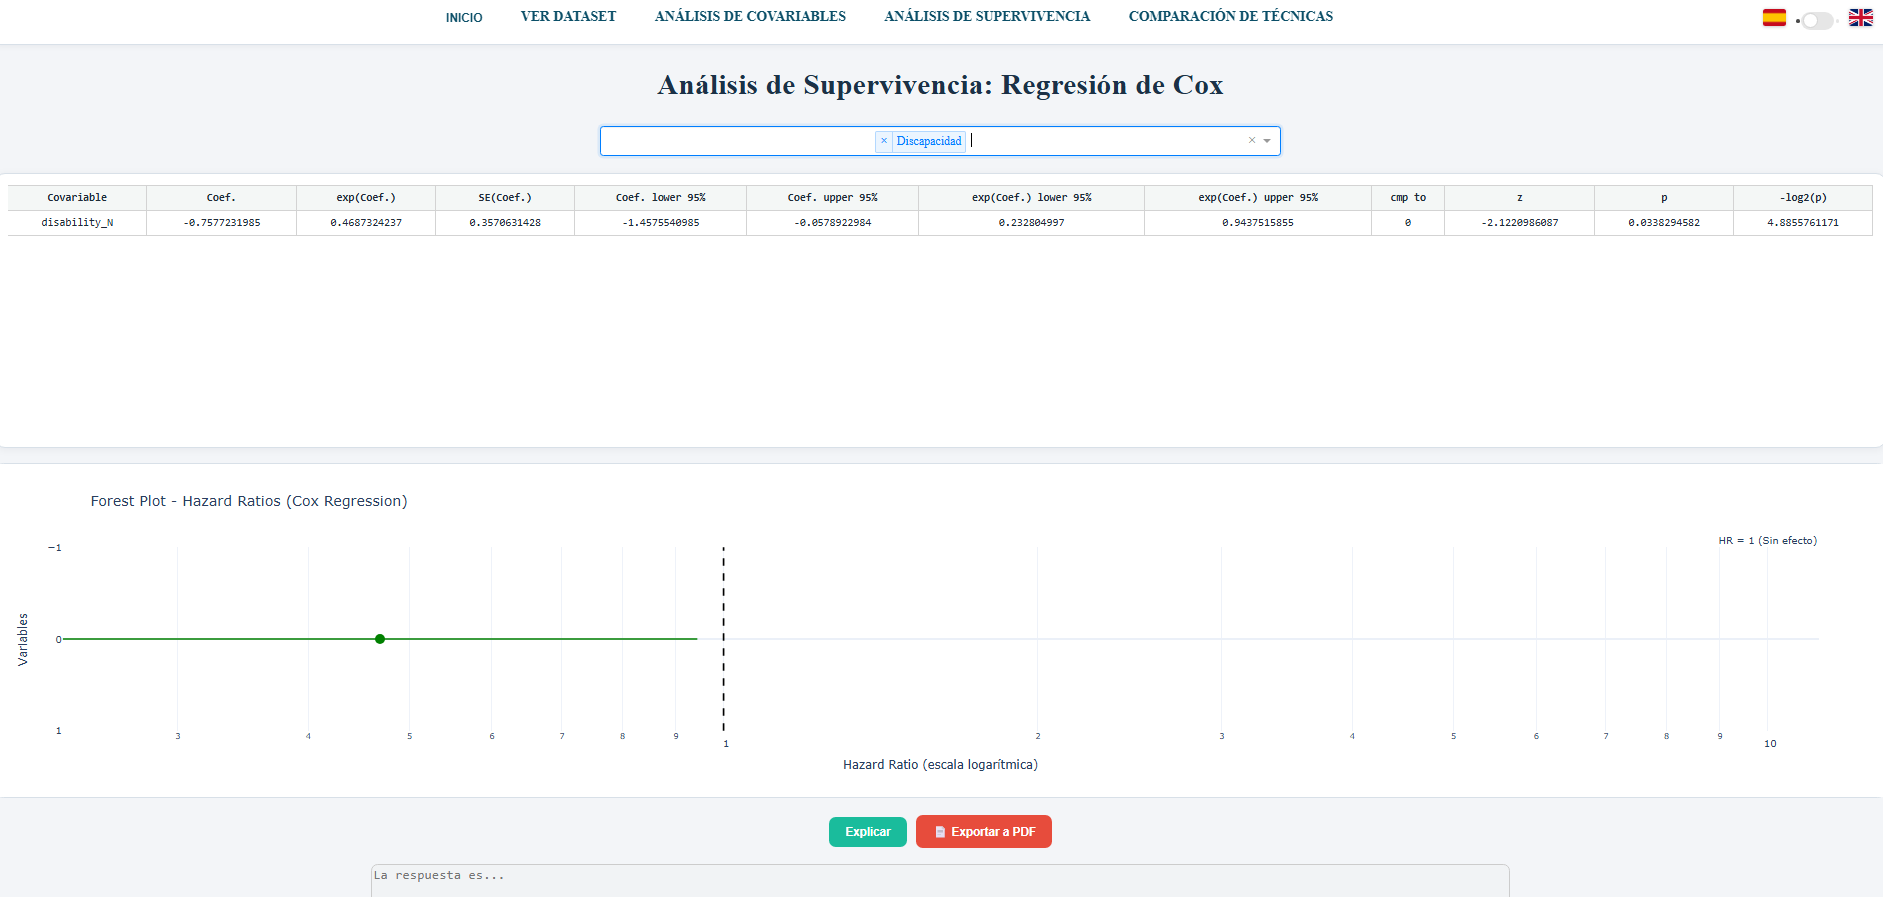
\includegraphics[width=\textwidth]{Imagenes/graficaCox.png}
    \caption{Gráfica generada a partir del modelo de regresión de Cox}
    \label{fig:interfaz_grafica_cox}
\end{figure}

\begin{figure}[H]
    \centering
    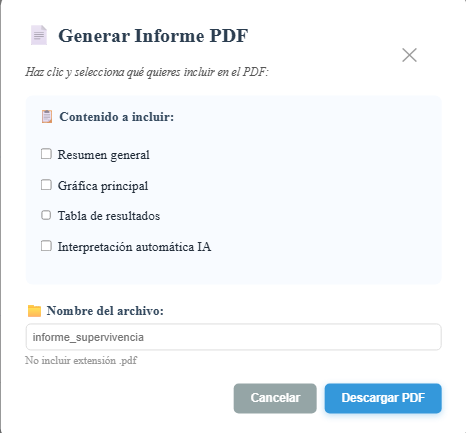
\includegraphics[width=0.4\textwidth]{Imagenes/botonPDFCox.png}
    \caption{Botón de exportación a PDF utilizado en Cox y también en el Test de Log-Rank}
    \label{fig:interfaz_boton_pdf_cox_logrank}
\end{figure}

\subsubsection*{\underline{Test de Log-Rank}}

\paragraph*{}
El Test de Log-Rank se utiliza para comparar curvas de supervivencia entre grupos. En la aplicación comparte parte de la estructura visual con la regresión de Cox, especialmente en los filtros, pero orienta la salida a la comparación estadística entre categorías.

\begin{figure}[H]
    \centering
    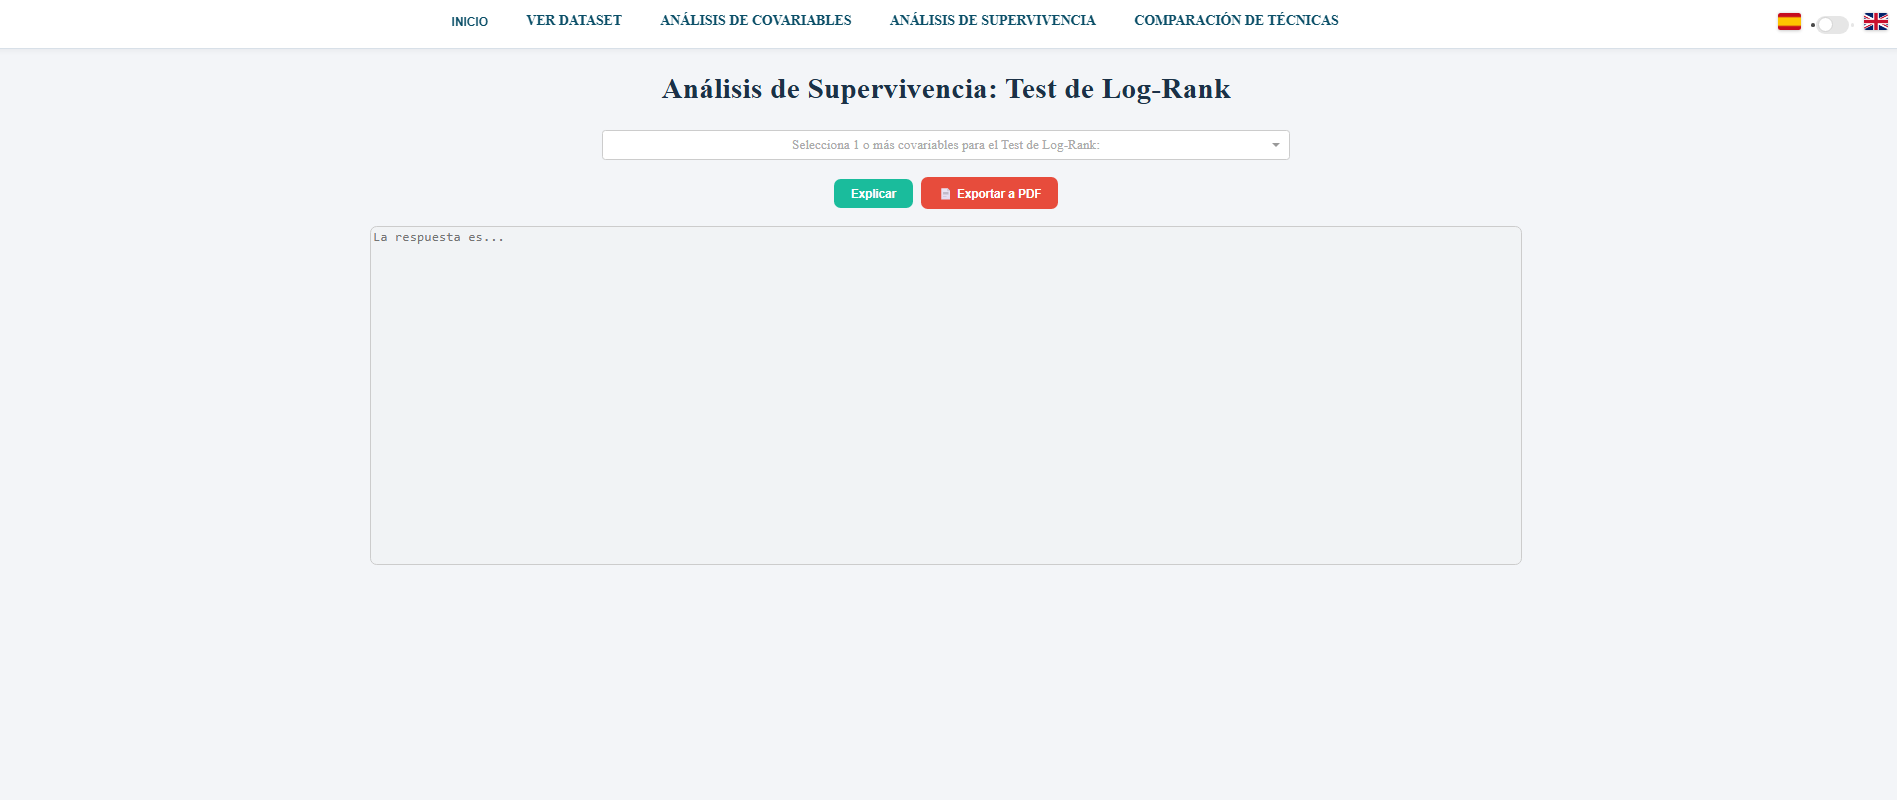
\includegraphics[width=\textwidth]{Imagenes/logRank.png}
    \caption{Vista principal del Test de Log-Rank}
    \label{fig:interfaz_logrank}
\end{figure}

\begin{figure}[H]
    \centering
    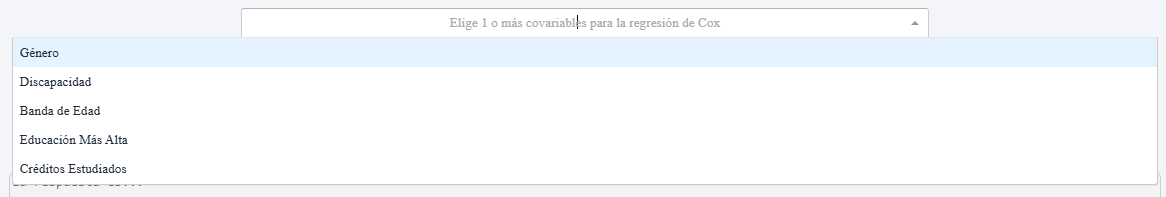
\includegraphics[width=\textwidth]{Imagenes/filtrosCox.png}
    \caption{Filtros compartidos por Cox y el Test de Log-Rank}
    \label{fig:interfaz_filtros_logrank}
\end{figure}

\begin{figure}[H]
    \centering
    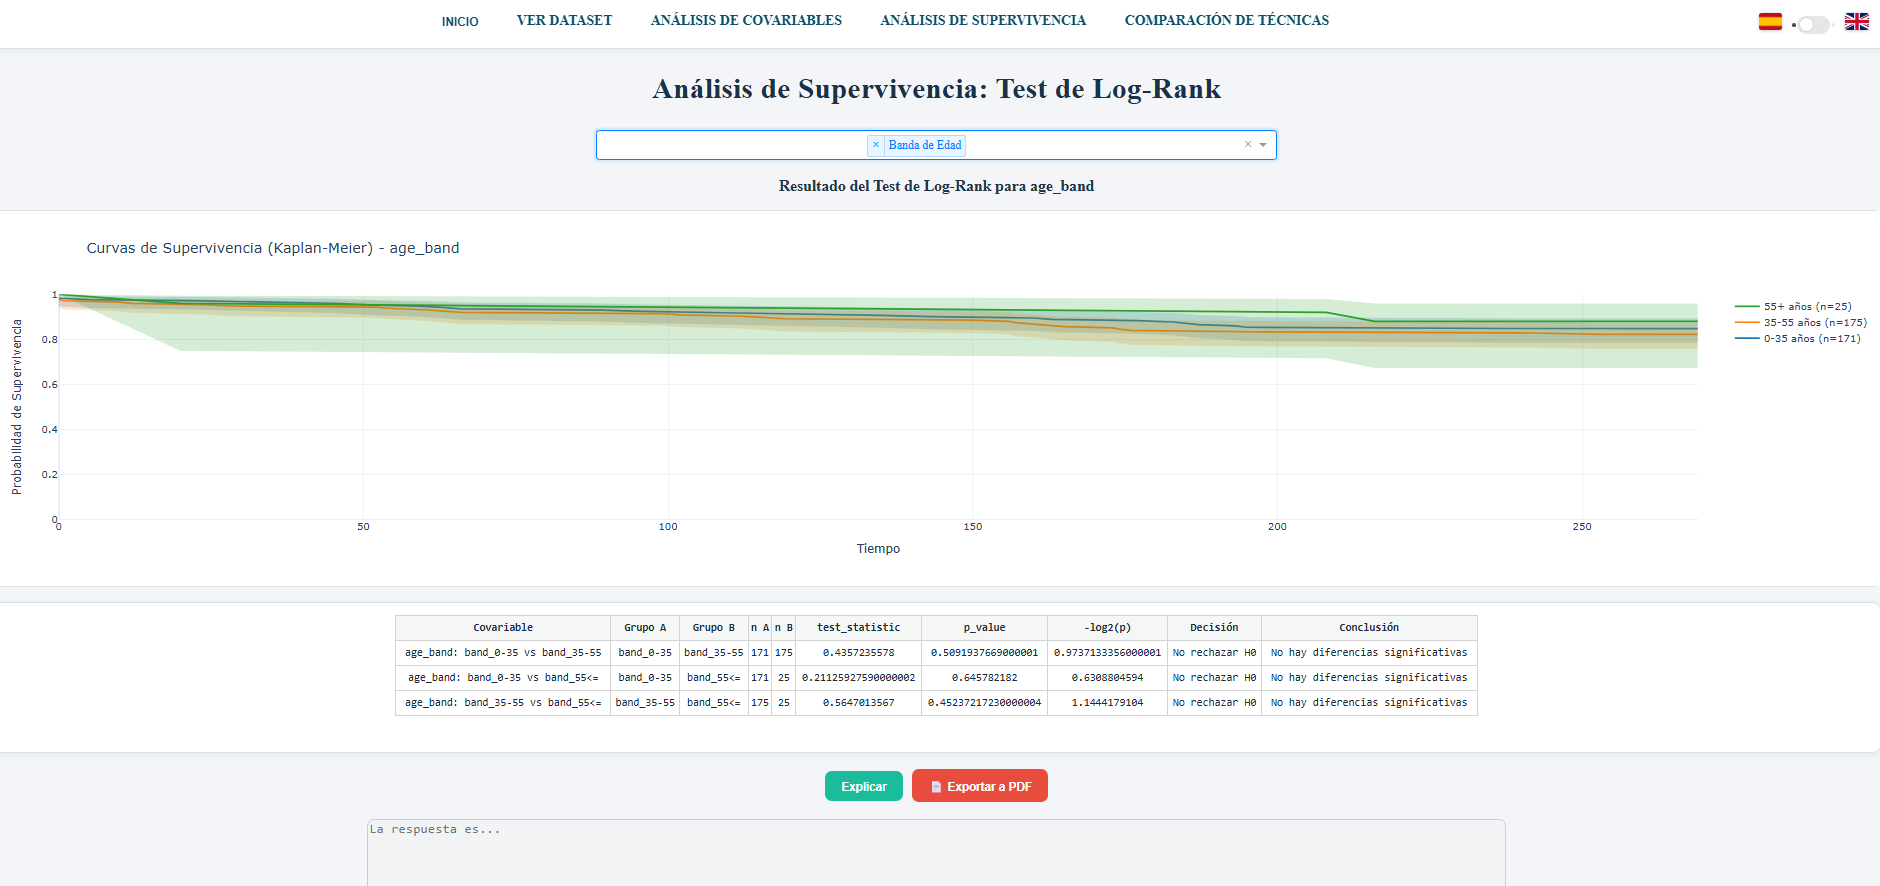
\includegraphics[width=\textwidth]{Imagenes/ejemploLogRank.png}
    \caption{Ejemplo de resultado generado mediante el Test de Log-Rank}
    \label{fig:interfaz_ejemplo_logrank}compilame de nuevo la documentacion para ver los nuevos cambios
\end{figure}

\subsubsection*{\underline{Weibull}}

\paragraph*{}
La técnica de Weibull amplía el análisis de supervivencia con un modelo paramétrico capaz de representar distintos comportamientos del riesgo a lo largo del tiempo. En la interfaz se muestran los resultados principales del ajuste, las visualizaciones asociadas y la opción de exportación conjunta.

\begin{figure}[H]
    \centering
    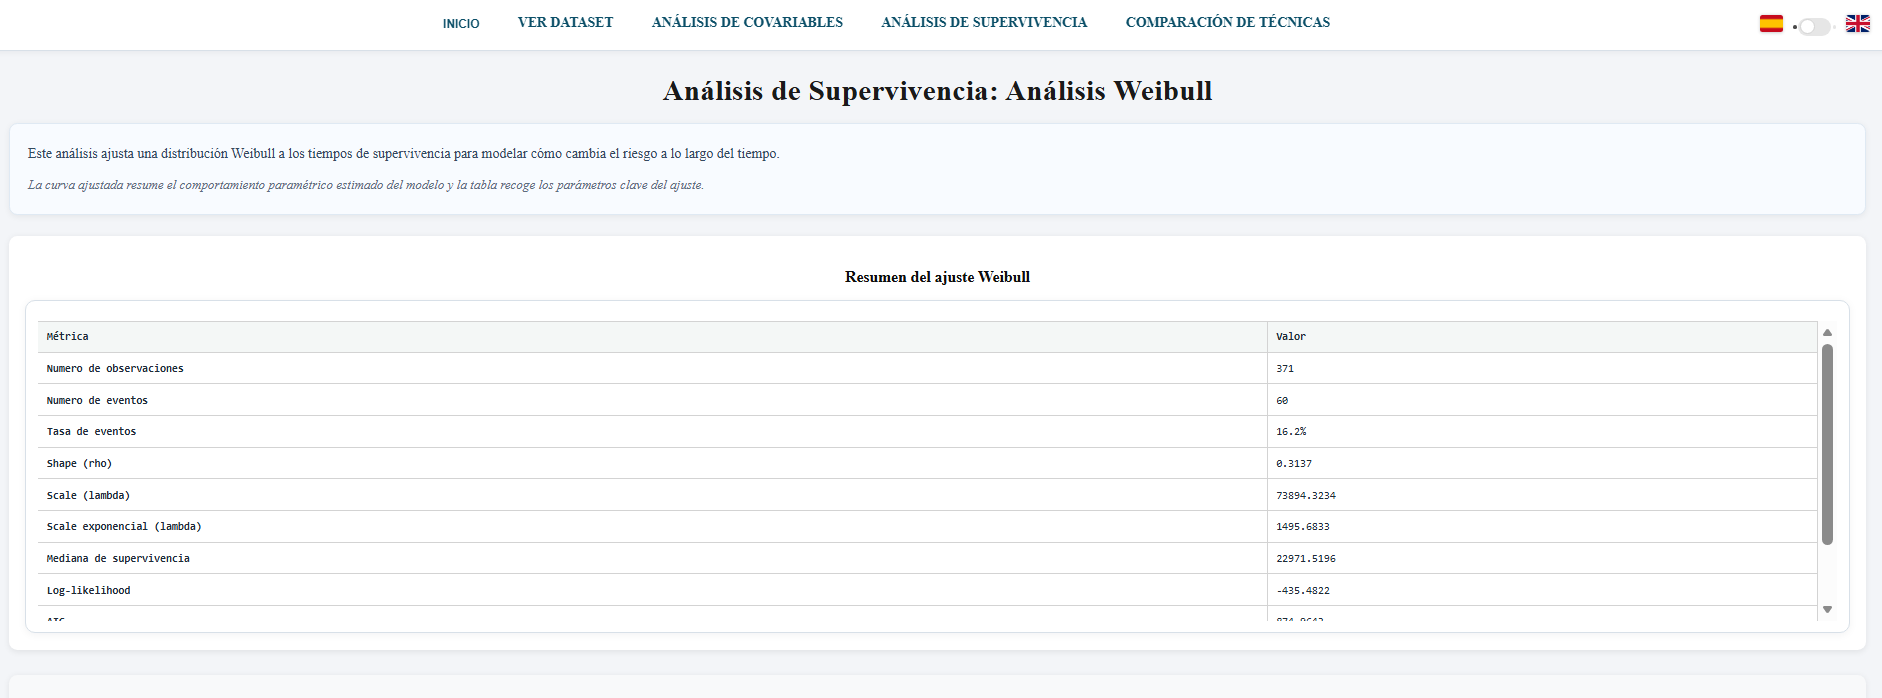
\includegraphics[width=\textwidth]{Imagenes/weibull1.png}
    \caption{Vista inicial del análisis mediante el modelo de Weibull}
    \label{fig:interfaz_weibull_1}
\end{figure}

\begin{figure}[H]
    \centering
    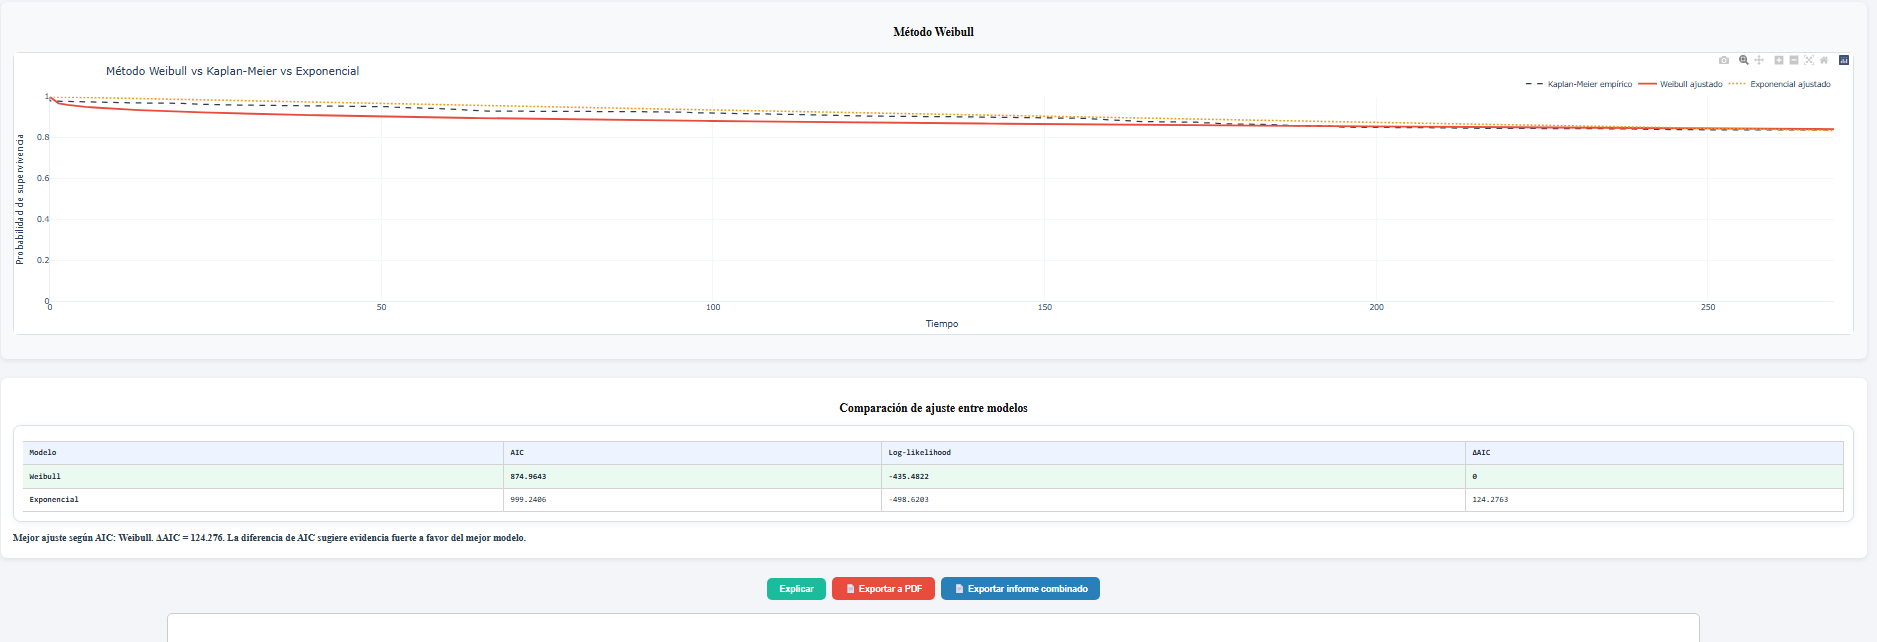
\includegraphics[width=\textwidth]{Imagenes/weibull2.png}
    \caption{Resultados y visualizaciones del modelo de Weibull}
    \label{fig:interfaz_weibull_2}
\end{figure}

\begin{figure}[H]
    \centering
    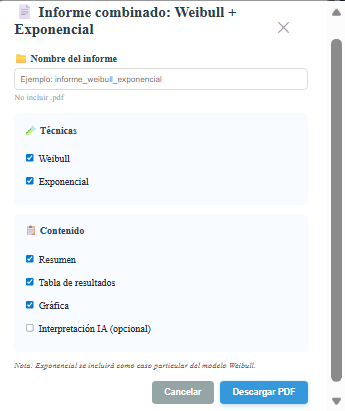
\includegraphics[width=\textwidth]{Imagenes/exportarCombinado.png}
    \caption{Botón de exportación combinada utilizado en Weibull y Exponencial, ya que ambos modelos exportan el mismo tipo de resultados}
    \label{fig:interfaz_exportar_combinado_weibull_exponencial}
\end{figure}

\subsubsection*{\underline{Exponencial}}

\paragraph*{}
El modelo exponencial ofrece una aproximación paramétrica más sencilla, basada en una tasa de riesgo constante. Por eso, dentro de la aplicación resulta útil como técnica de referencia, especialmente para comparar su comportamiento frente a modelos más flexibles como Weibull o Random Survival Forest.

\begin{figure}[H]
    \centering
    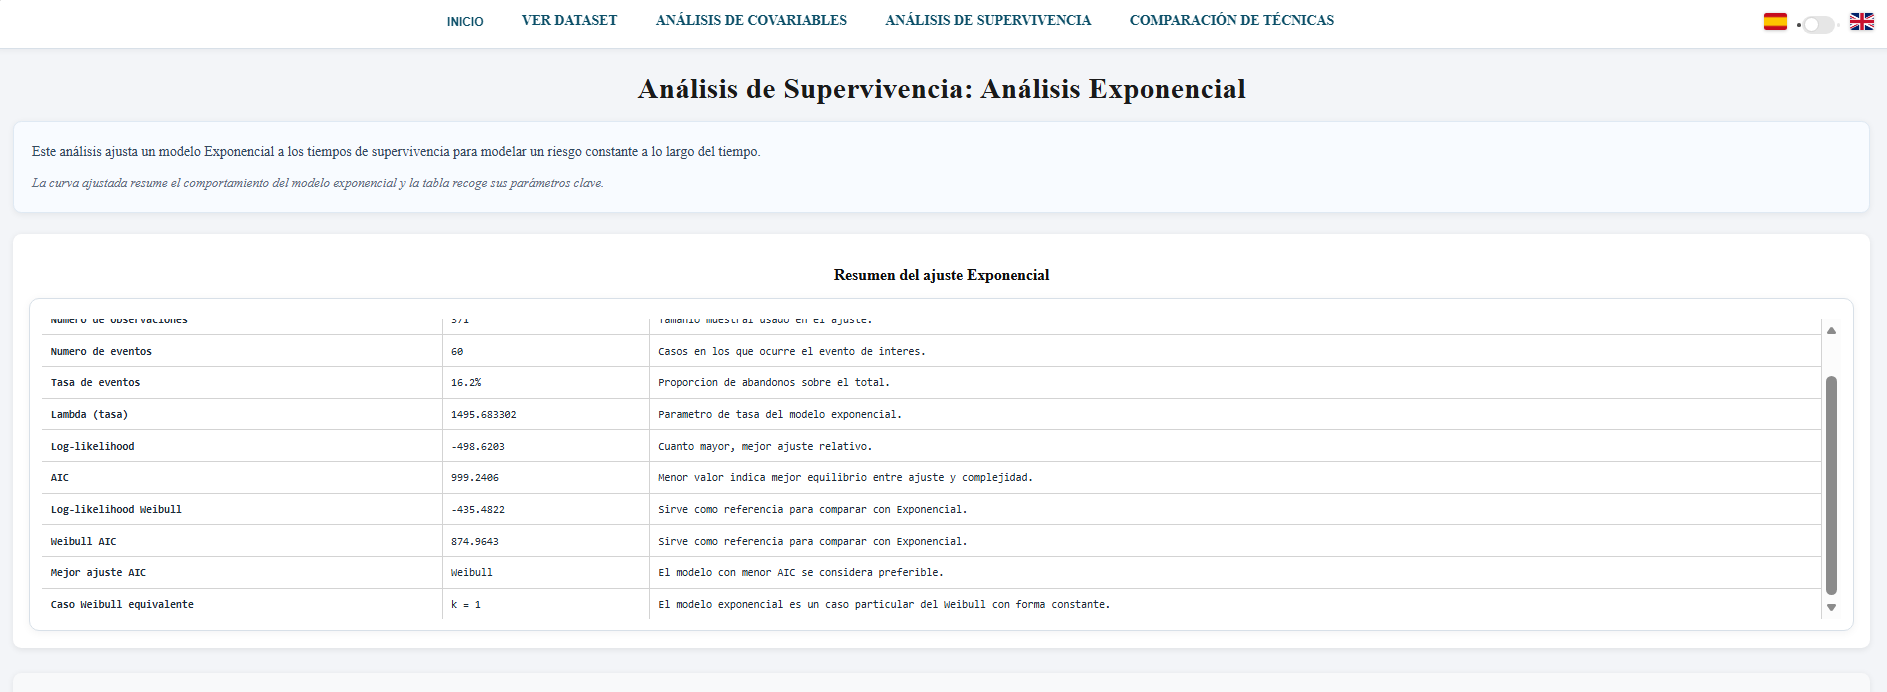
\includegraphics[width=\textwidth]{Imagenes/exponencial1.png}
    \caption{Vista inicial del análisis mediante el modelo exponencial}
    \label{fig:interfaz_exponencial_1}
\end{figure}

\begin{figure}[H]
    \centering
    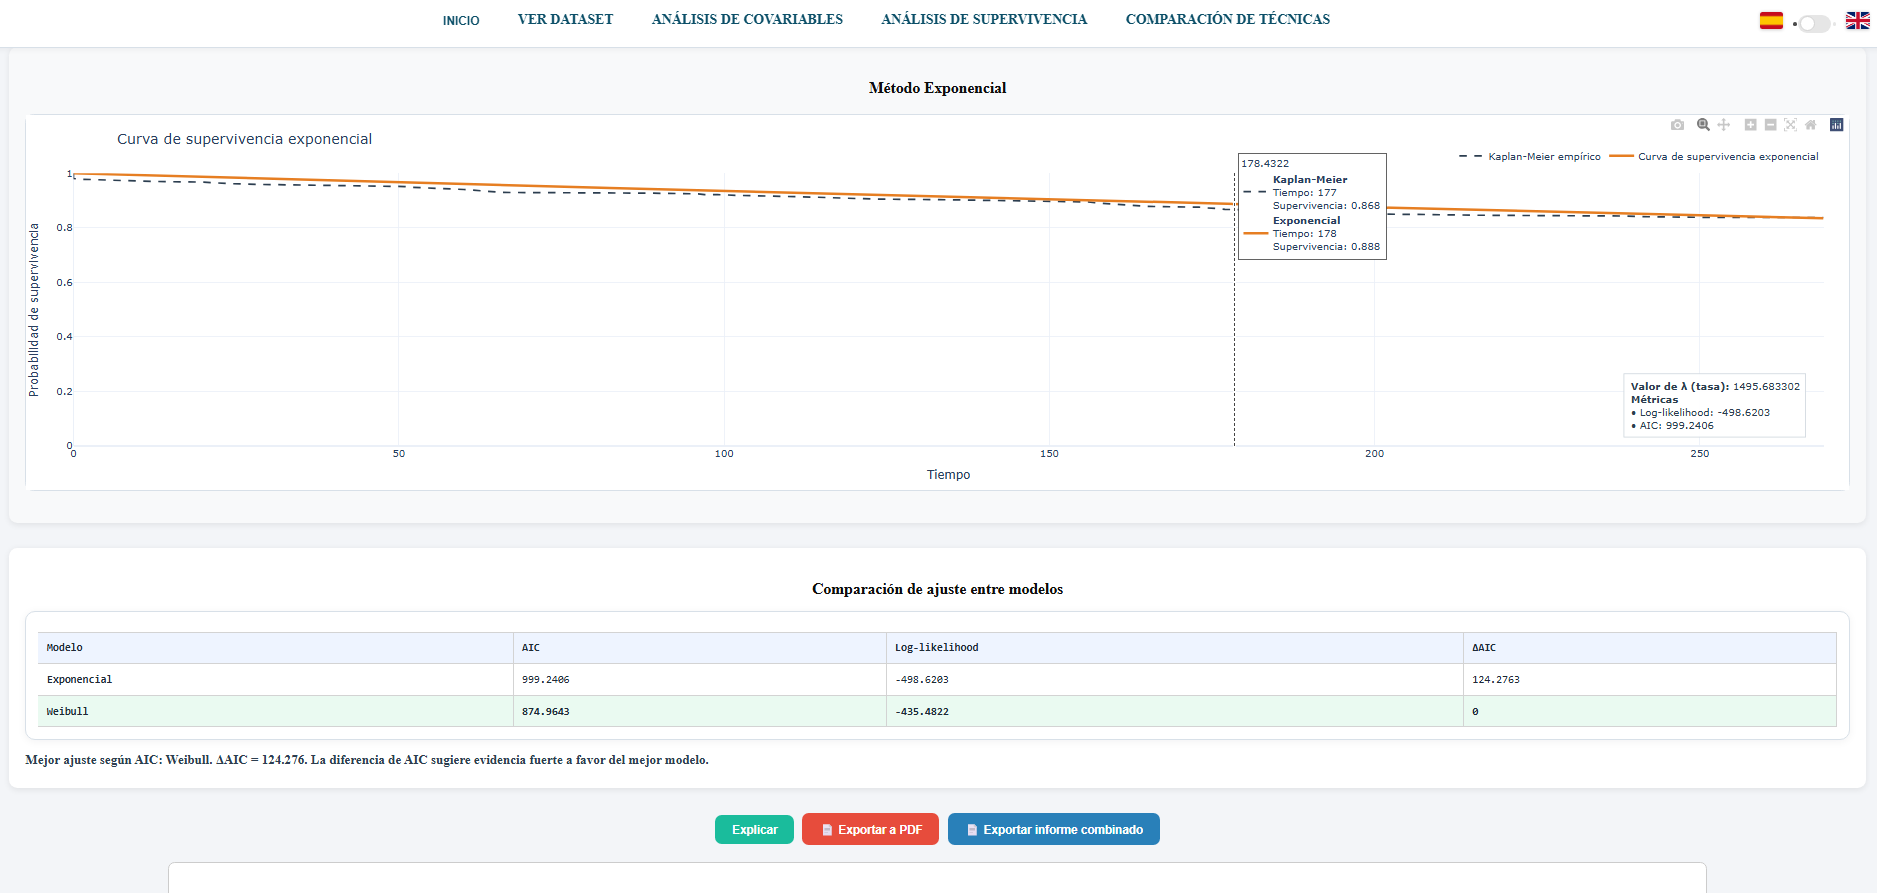
\includegraphics[width=\textwidth]{Imagenes/exponencial2.png}
    \caption{Resultados y visualizaciones del modelo exponencial}
    \label{fig:interfaz_exponencial_2}
\end{figure}

\subsubsection*{\underline{Random Survival Forest}}

\paragraph*{}
Random Survival Forest incorpora una técnica basada en aprendizaje automático para estudiar relaciones más complejas entre las variables del dataset y el tiempo hasta el evento. La interfaz recoge tanto la ejecución del modelo como los resultados gráficos y métricos necesarios para interpretar su comportamiento.

\begin{figure}[H]
    \centering
    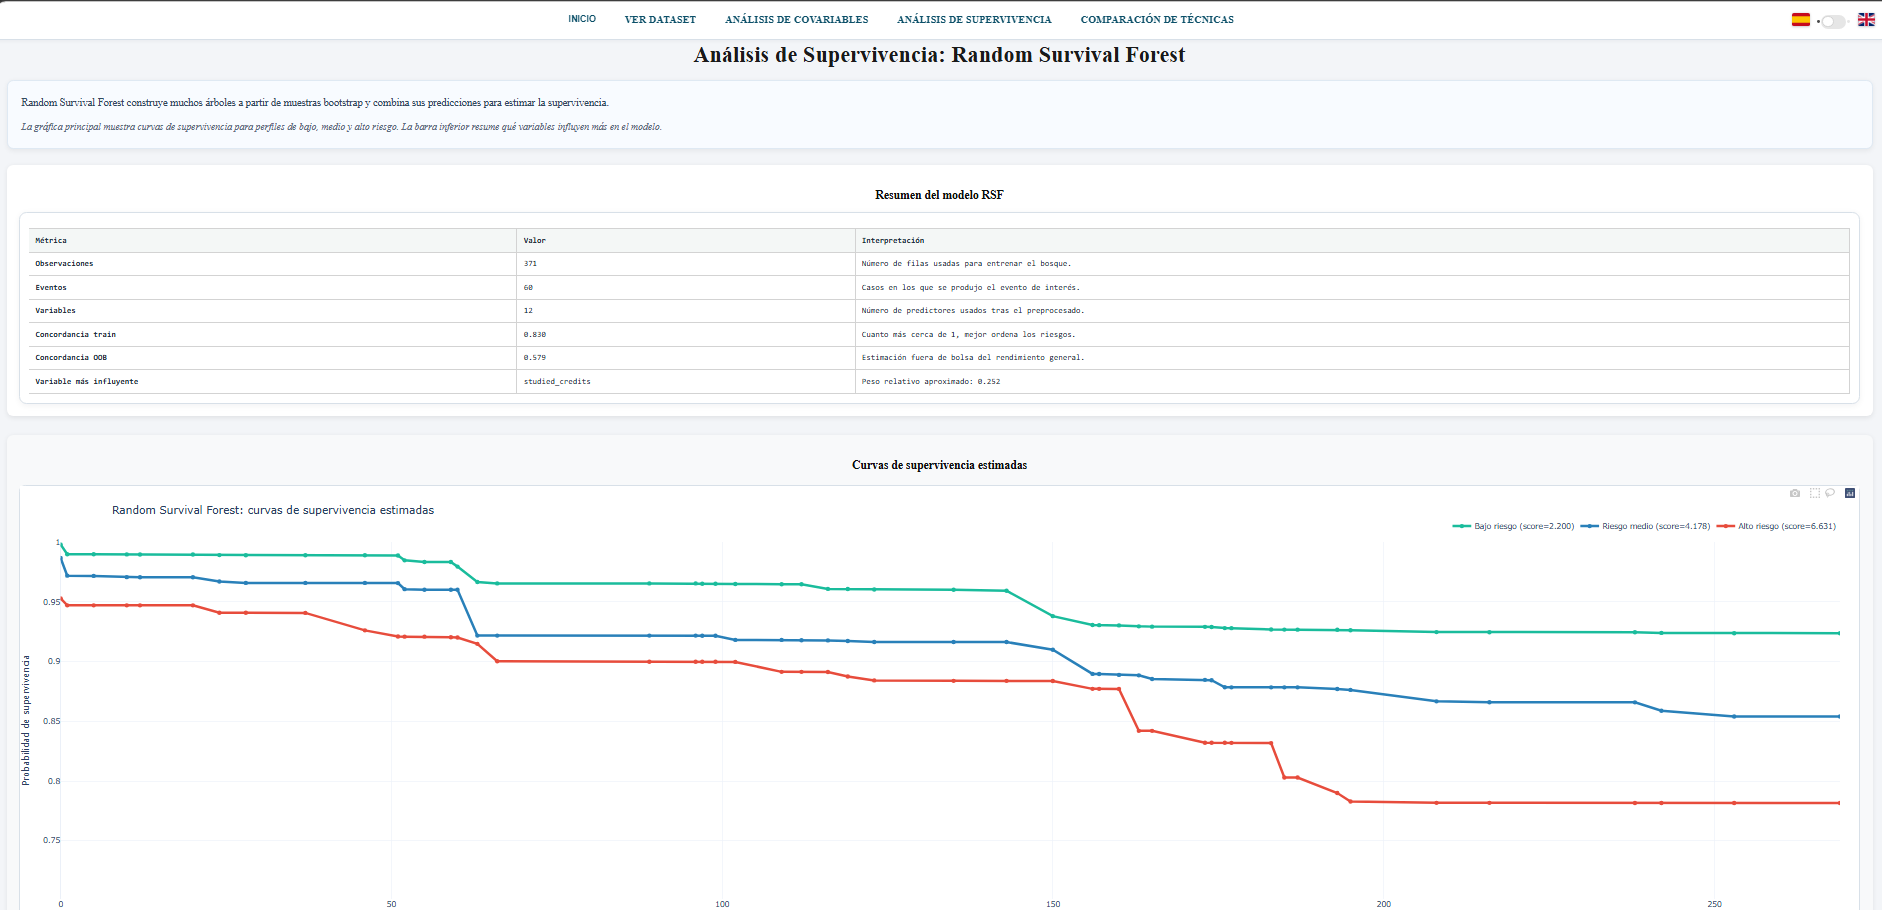
\includegraphics[width=\textwidth]{Imagenes/rsf1.png}
    \caption{Vista inicial del análisis mediante Random Survival Forest}
    \label{fig:interfaz_rsf_1}
\end{figure}

\begin{figure}[H]
    \centering
    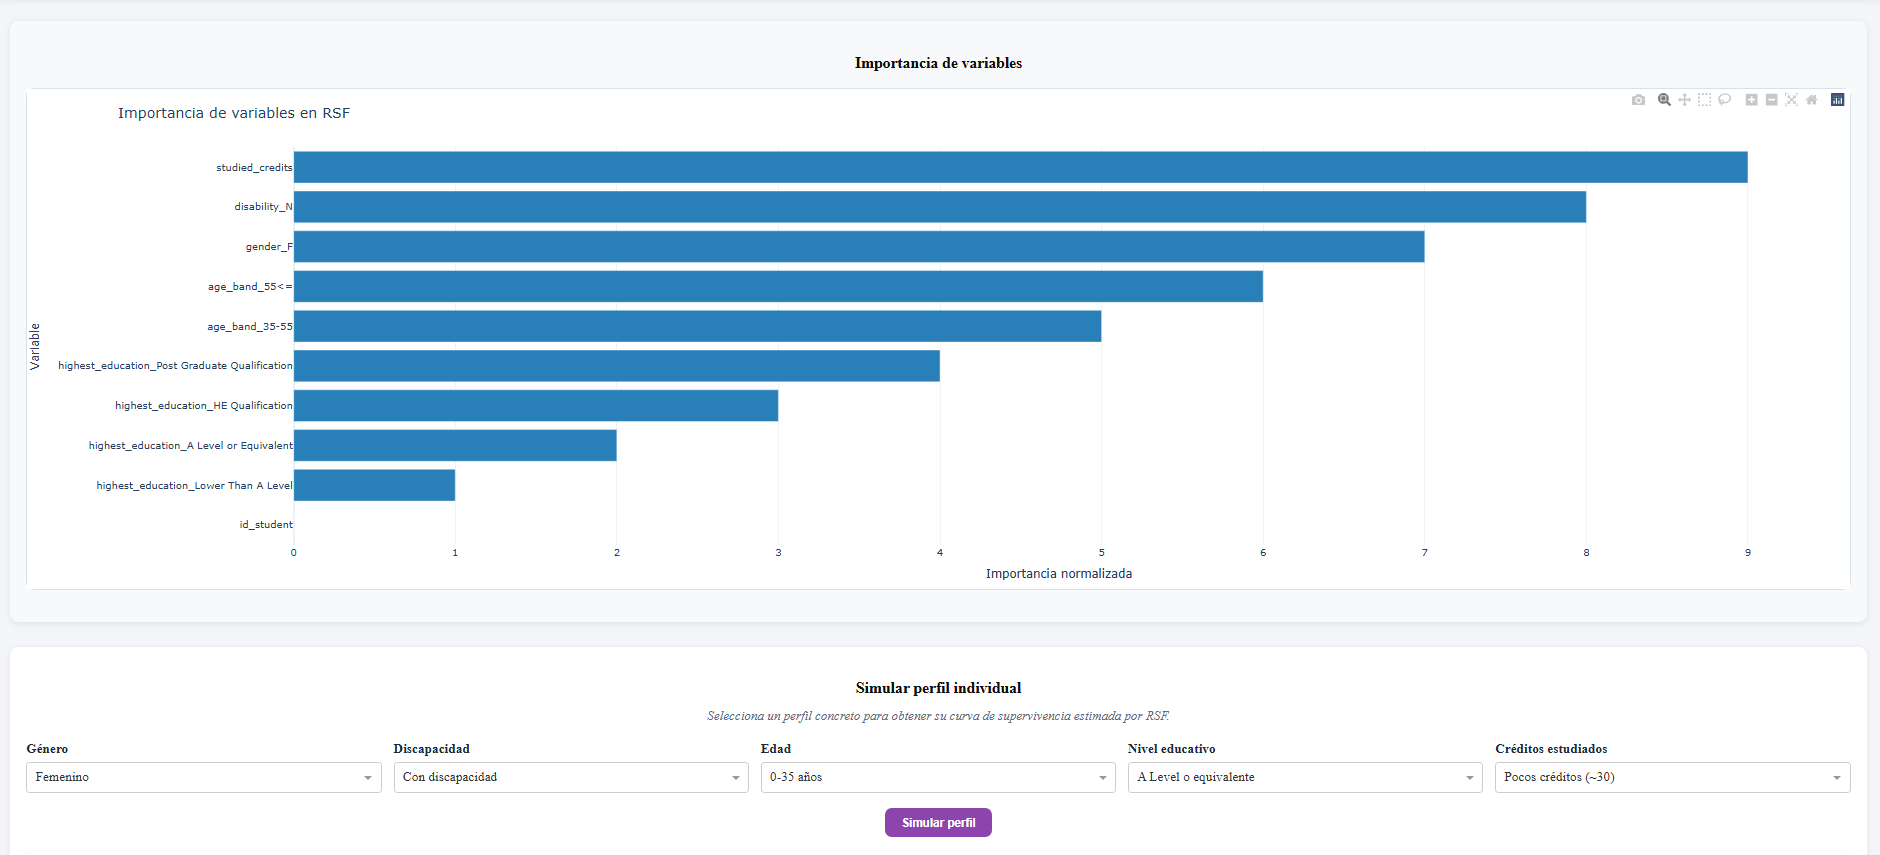
\includegraphics[width=\textwidth]{Imagenes/rsf2.png}
    \caption{Resultados generales generados por Random Survival Forest}
    \label{fig:interfaz_rsf_2}
\end{figure}

\begin{figure}[H]
    \centering
    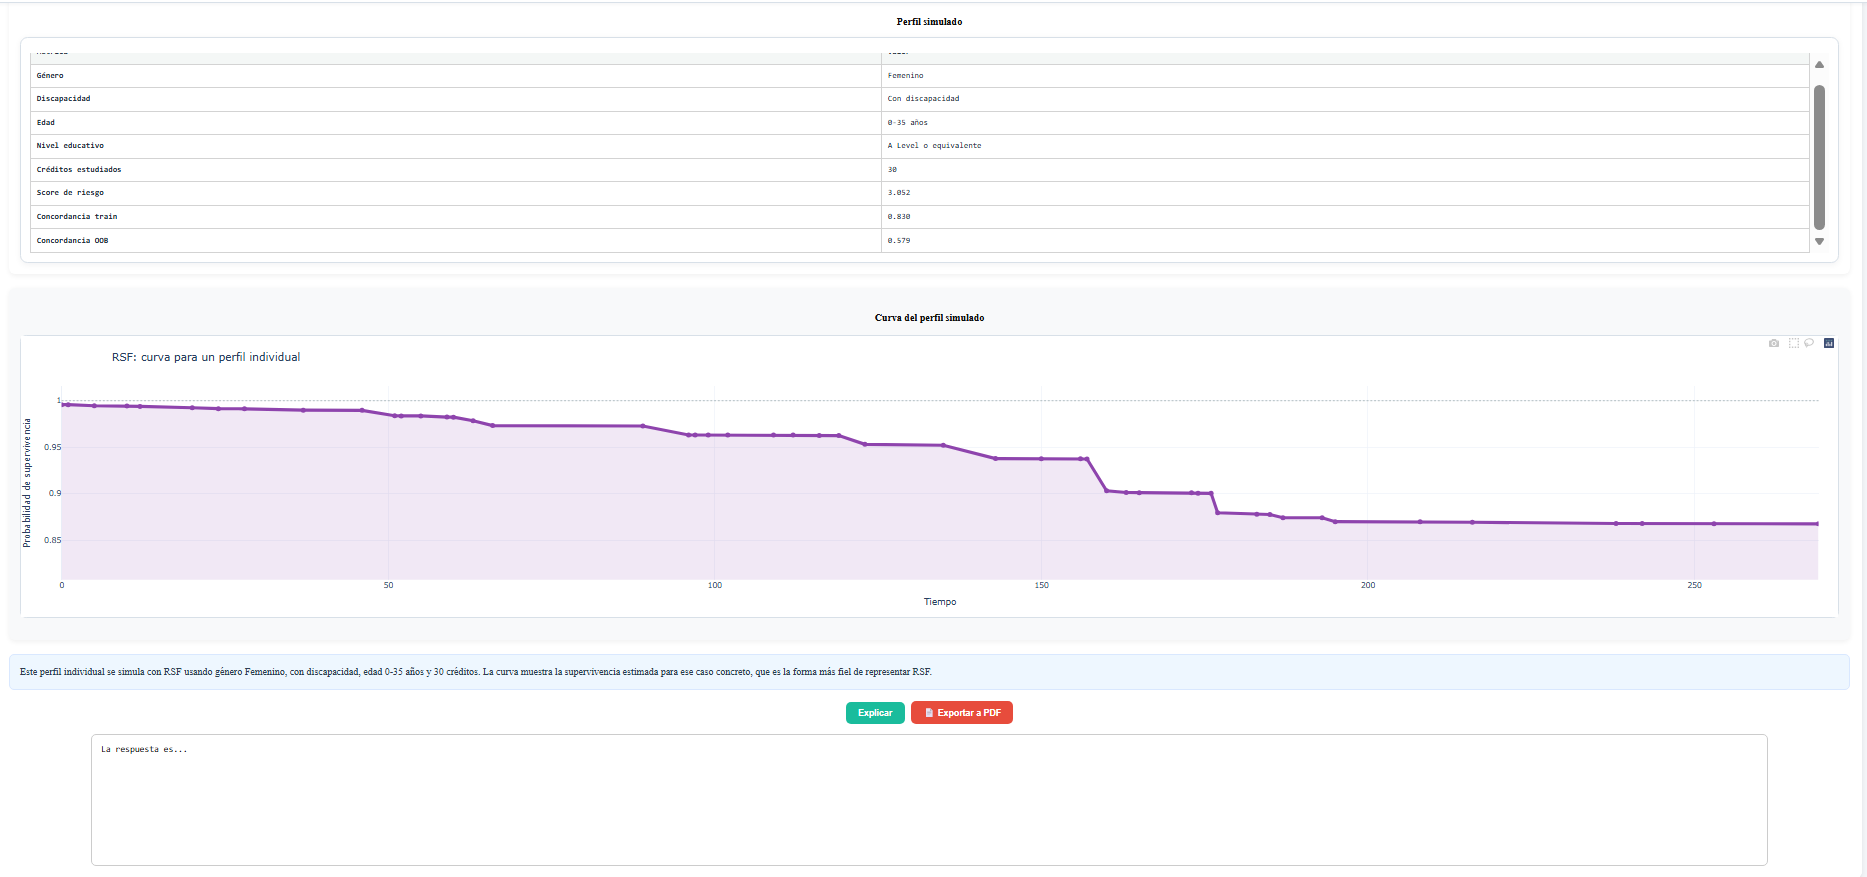
\includegraphics[width=\textwidth]{Imagenes/rsf3.png}
    \caption{Visualización complementaria del análisis Random Survival Forest}
    \label{fig:interfaz_rsf_3}
\end{figure}

\subsubsection*{\underline{Comparación de técnicas}}

\paragraph*{}
La página de comparación de técnicas se abre desde el botón específico situado bajo las técnicas de la sección de análisis de supervivencia. A diferencia de las vistas anteriores, no se trata de un modelo ejecutable, sino de una página estática pensada para orientar al usuario. En ella se resume, de forma sencilla, qué hace cada método, qué tipo de información aporta y en qué situaciones puede resultar más útil. La idea es que el usuario no tenga que elegir una técnica a ciegas, sino que cuente con una pequeña guía dentro de la propia aplicación.

\begin{figure}[H]
    \centering
    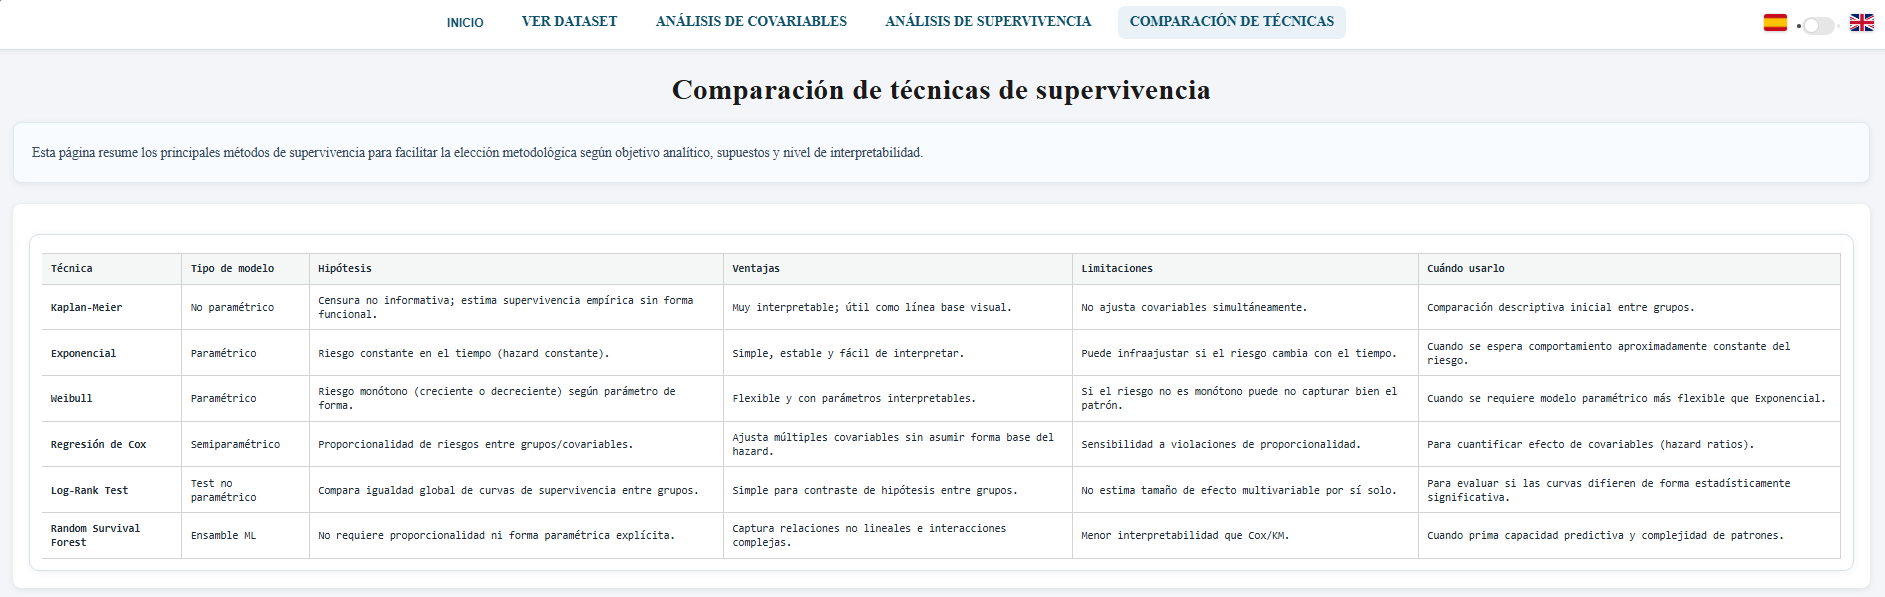
\includegraphics[width=\textwidth]{Imagenes/comparar1.png}
    \caption{Página de comparación de técnicas de supervivencia}
    \label{fig:interfaz_comparar_tecnicas_1}
\end{figure}

\begin{figure}[H]
    \centering
    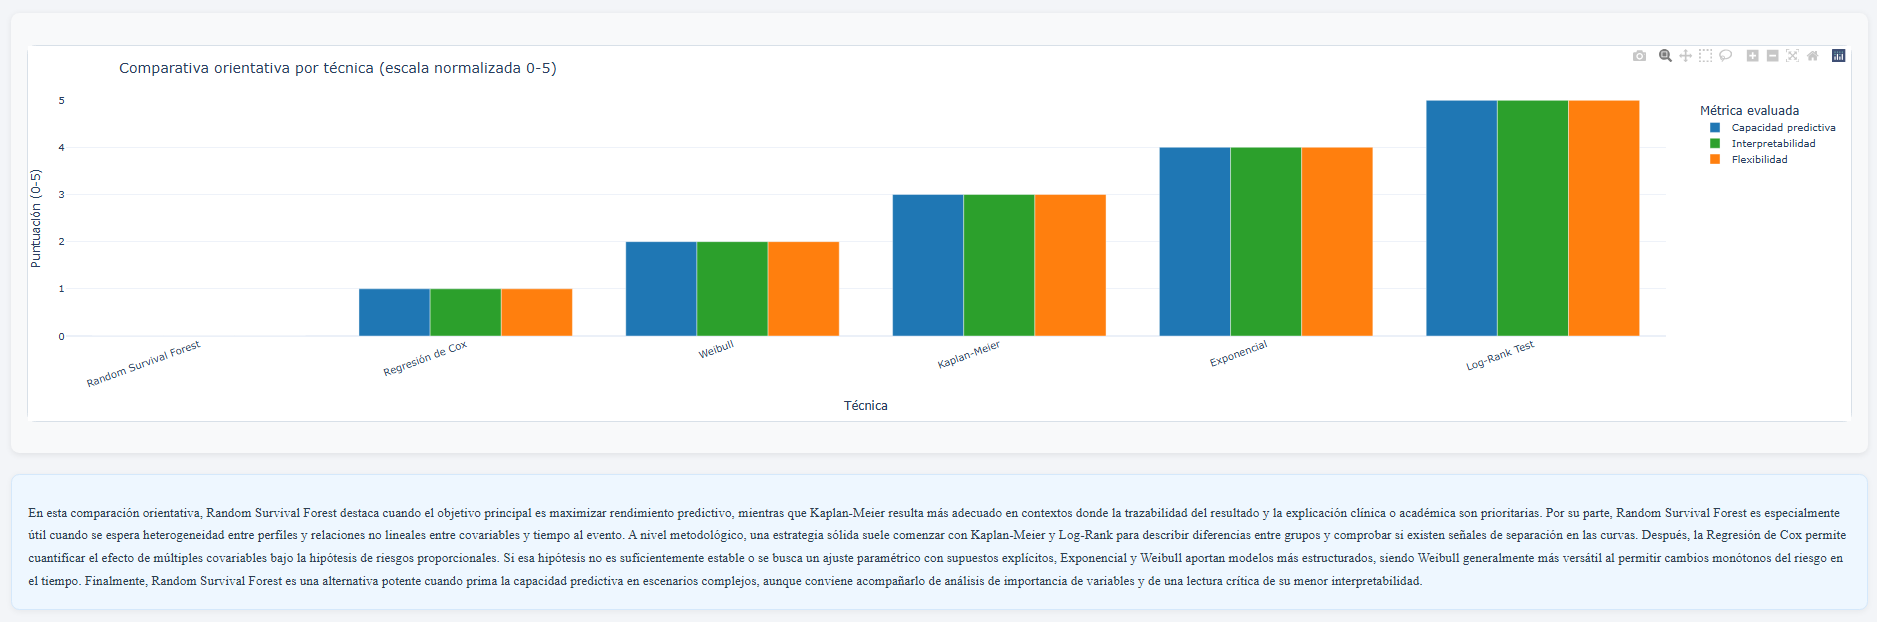
\includegraphics[width=\textwidth]{Imagenes/comparar2.png}
    \caption{Detalle explicativo de la comparación de técnicas}
    \label{fig:interfaz_comparar_tecnicas_2}
\end{figure}

\subsubsection*{\underline{Botones}}

\paragraph*{}
La interfaz incluye distintos botones de acción que guían al usuario durante el uso de la aplicación. Algunos permiten cambiar entre vistas del dataset, otros activan funcionalidades de apoyo como la interpretación mediante inteligencia artificial, y otros se encargan de la exportación de resultados. Aunque son elementos pequeños dentro de la pantalla, la verdad es que tienen bastante peso en la experiencia de uso, porque marcan los pasos principales del flujo de trabajo.

\begin{figure}[H]
    \centering
    
\includegraphics[width=0.45\textwidth]{Imagenes/botonInicio.png}
    \caption{Botón para consultar el dataset bruto}
    \label{fig:interfaz_boton_inicio}
\end{figure}

\begin{figure}[H]
    \centering
    
\includegraphics[width=0.45\textwidth]{Imagenes/botonYaLimpio.png}
    \caption{Botón para consultar el dataset limpio}
    \label{fig:interfaz_boton_dataset_limpio}
\end{figure}

\begin{figure}[H]
    \centering
    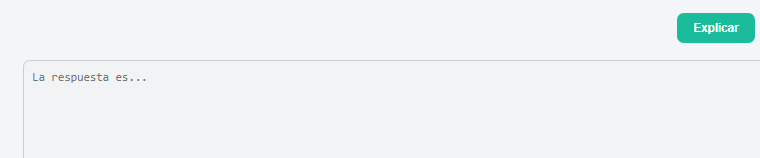
\includegraphics[width=0.45\textwidth]{Imagenes/botonIA.png}
    \caption{Botón para solicitar una interpretación mediante inteligencia artificial}
    \label{fig:interfaz_boton_ia}
\end{figure}

\begin{figure}[H]
    \centering
    
\includegraphics[width=0.45\textwidth]{Imagenes/botonExportar.png}
    \caption{Botón de exportación de resultados}
    \label{fig:interfaz_boton_exportar}
\end{figure}

\paragraph*{}
Al pulsar el botón de exportación se abre una ventana modal en la que el usuario puede seleccionar la opción de generar informe. Una vez confirmada la acción, el sistema prepara el documento y se descarga el PDF correspondiente.

\begin{figure}[H]
    \centering
    
\includegraphics[width=0.45\textwidth]{Imagenes/botonDentroexportar.png}
    \caption{Botón de confirmación para generar y descargar el informe PDF}
    \label{fig:interfaz_boton_dentro_exportar}
\end{figure}

\paragraph*{}
En los modelos Weibull y Exponencial se incluye además un botón de exportación combinada, ya que ambos representan una relación de caso general y caso particular dentro de los modelos paramétricos. Por su parte, Random Survival Forest incorpora un botón específico para simular perfiles, lo que permite explorar el comportamiento del modelo ante distintas combinaciones de variables.

\begin{figure}[H]
    \centering
    
\includegraphics[width=0.45\textwidth]{Imagenes/botonCombinado.png}
    \caption{Botón de exportación combinada para Weibull y Exponencial}
    \label{fig:interfaz_boton_combinado}
\end{figure}

\begin{figure}[H]
    \centering
    
\includegraphics[width=0.45\textwidth]{Imagenes/botonSimularPerfil.png}
    \caption{Botón de simulación de perfiles en Random Survival Forest}
    \label{fig:interfaz_boton_simular_perfil}
\end{figure}

\section{Diagrama de clases y componentes}

\paragraph*{}
Al tratarse de una aplicación desarrollada principalmente con Dash, funciones de Python y callbacks, el sistema no sigue una estructura clásica basada únicamente en clases. Por ese motivo, en este apartado se plantea una vista mixta de clases y componentes, donde se representan tanto la clase principal de exportación como los módulos funcionales que sostienen el comportamiento del dashboard. Esta visión resulta más fiel al proyecto que forzar un diagrama de clases tradicional con entidades que realmente no existen en el código.

\paragraph*{}
El componente central es la aplicación Dash, que actúa como núcleo de ejecución y como punto de conexión entre la interfaz, la navegación y los callbacks. A partir de ella se coordinan los componentes visuales y las respuestas del sistema ante las acciones del usuario. Por ejemplo, cuando se selecciona una técnica de análisis, el sistema recupera el dataset preparado, ejecuta el modelo correspondiente y devuelve a la interfaz los resultados que deben mostrarse.

\paragraph*{}
En cuanto a clases propiamente dichas, destaca la clase responsable de construir los informes PDF. Esta clase concentra la creación del documento final, añadiendo secciones, tablas, gráficas e interpretaciones. Su existencia tiene sentido porque la generación de informes requiere mantener una estructura interna y reutilizar operaciones comunes en distintos tipos de salida. Los detalles concretos de esta clase y de los archivos implicados se describen en el capítulo de implementación.

\begin{table}[H]
\centering
\small
\begin{tabular}{|p{0.38\textwidth}|p{0.52\textwidth}|}
\hline
\textbf{Elemento de diseño} & \textbf{Descripción} \\ \hline
\texttt{Dash App} & Núcleo de la aplicación web. Gestiona la ejecución del servidor local y la navegación entre páginas. \\ \hline
\texttt{Layouts} & Componentes visuales creados en \texttt{layout.py}. Definen qué ve el usuario en cada pantalla. \\ \hline
\texttt{Callbacks de análisis} & Funciones que responden a eventos de la interfaz y conectan la entrada del usuario con los modelos estadísticos. \\ \hline
\texttt{Módulos de modelos} & Funciones específicas para Kaplan-Meier, Cox, Test de Log-Rank, Exponencial, Weibull y Random Survival Forest. \\ \hline
\texttt{Módulo IA} & Componente encargado de enviar información del análisis al modelo local y recuperar una explicación textual. \\ \hline
\texttt{SurvivalAnalysisPDF}\\ \texttt{Exporter} & Clase responsable de generar informes PDF reutilizando tablas, gráficos e interpretaciones. \\ \hline
\texttt{Traducciones} & Diccionario de textos que permite adaptar la interfaz al idioma seleccionado. \\ \hline
\end{tabular}
\caption{Vista de diseño basada en clases y componentes del sistema}
\label{tab:componentes_diseno}
\end{table}

\begin{figure}[H]
    \centering
    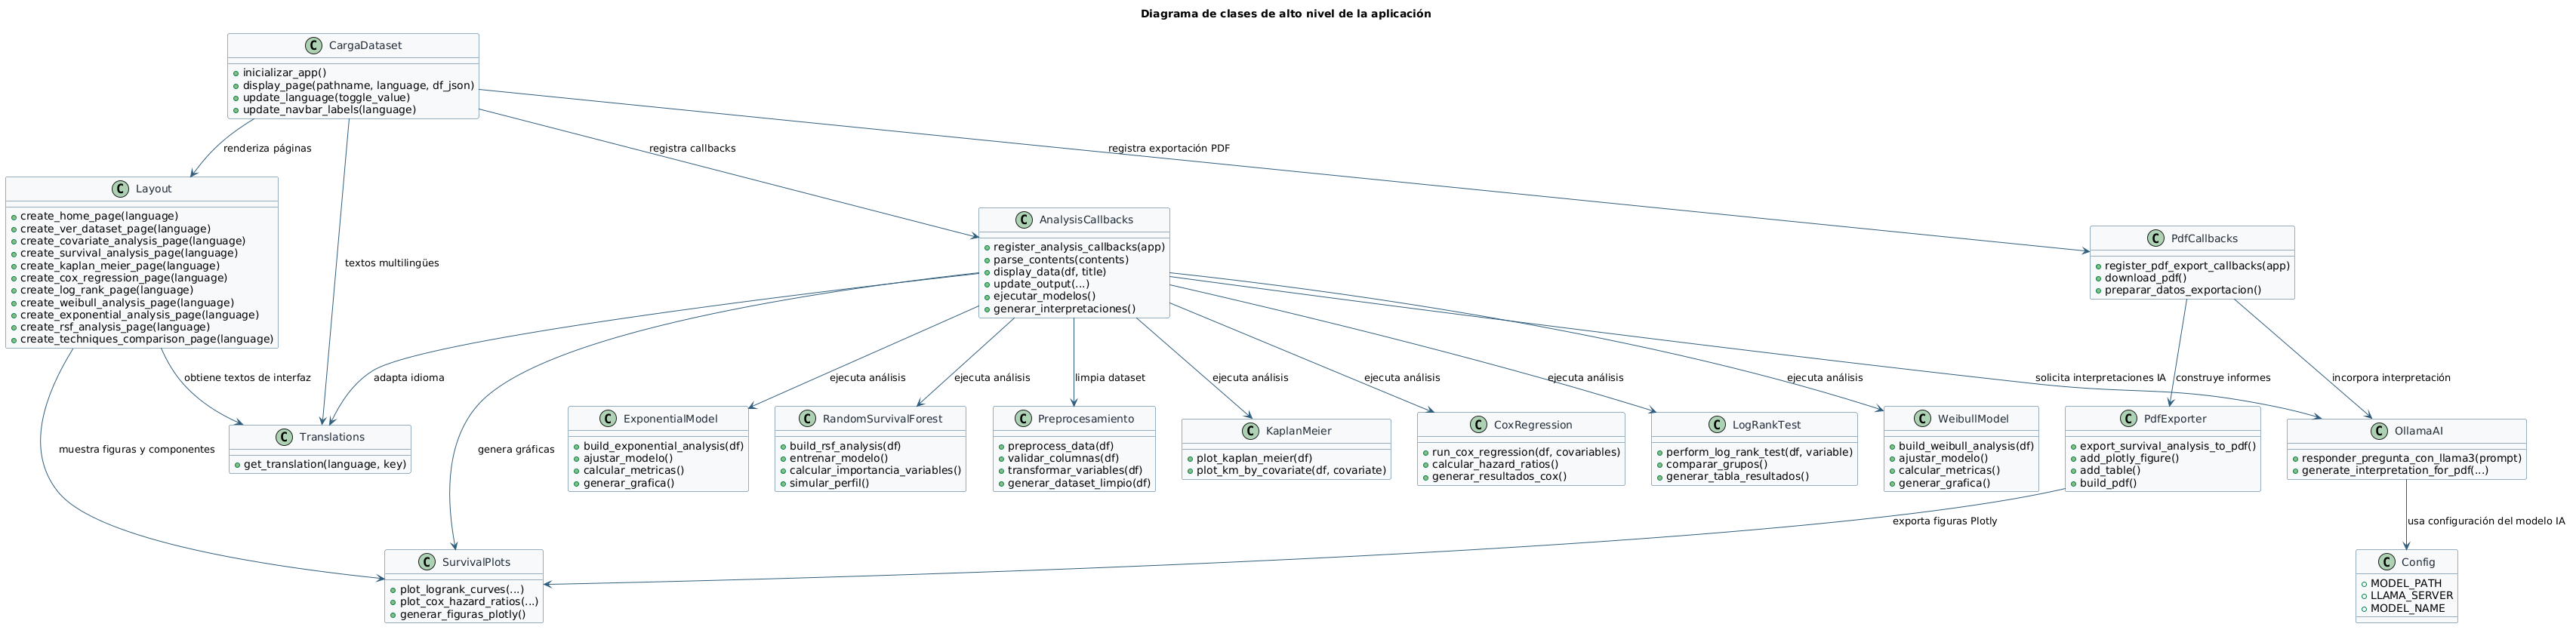
\includegraphics[width=0.95\textwidth,height=0.78\textheight,keepaspectratio]{Imagenes/diagrama_clases.png}
    \caption{Diagrama de clases y componentes de la aplicación}
    \label{fig:diagrama_clases_componentes}
\end{figure}

\section{Diagramas de secuencia}

\paragraph*{}
Los diagramas de secuencia muestran cómo colaboran los principales componentes del sistema cuando el usuario ejecuta cada una de las funcionalidades definidas en los casos de uso. A diferencia de los diagramas de actividad, que se centran en el flujo de acciones, estos diagramas ayudan a entender qué partes internas intervienen en cada proceso: la interfaz, los callbacks, el dataset, los modelos de análisis, la generación de visualizaciones, la inteligencia artificial o la exportación de informes.
\paragraph*{}
En los diagramas de secuencia se utiliza una nomenclatura descriptiva para facilitar la lectura de las interacciones. Por este motivo, algunos participantes aparecen con nombres funcionales, como ``Interfaz Dash'', ``Callbacks de análisis'' o ``Estado del dataset'', en lugar de emplear exactamente los nombres técnicos utilizados en la vista de clases y componentes. Estos participantes no deben interpretarse siempre como clases Python estrictas, sino como componentes o responsabilidades del sistema. No obstante, se corresponden con los elementos descritos anteriormente: la interfaz se relaciona con \texttt{DashApp} y \texttt{layout.py}, los callbacks con \texttt{AnalysisCallbacks}, el estado del dataset con el componente \texttt{Dataset}, y los módulos de análisis con sus correspondientes modelos.

\subsection{CU-1: EjecutarModeloExponencial}
\paragraph*{}
El diagrama de secuencia del CU-1 muestra cómo se coordina la interfaz con los callbacks de análisis para ejecutar el modelo exponencial. Primero se comprueba que el dataset esté cargado y preprocesado; si los datos son válidos, el sistema llama al módulo \texttt{exponential.py}, genera la gráfica mediante Plotly y devuelve al usuario la tabla resumen, la visualización y la comparativa de ajuste. Además, el diagrama incluye las interacciones opcionales con el módulo de IA y con la exportación a PDF, así como el camino alternativo cuando el dataset no es compatible.

\begin{figure}[H]
    \centering
    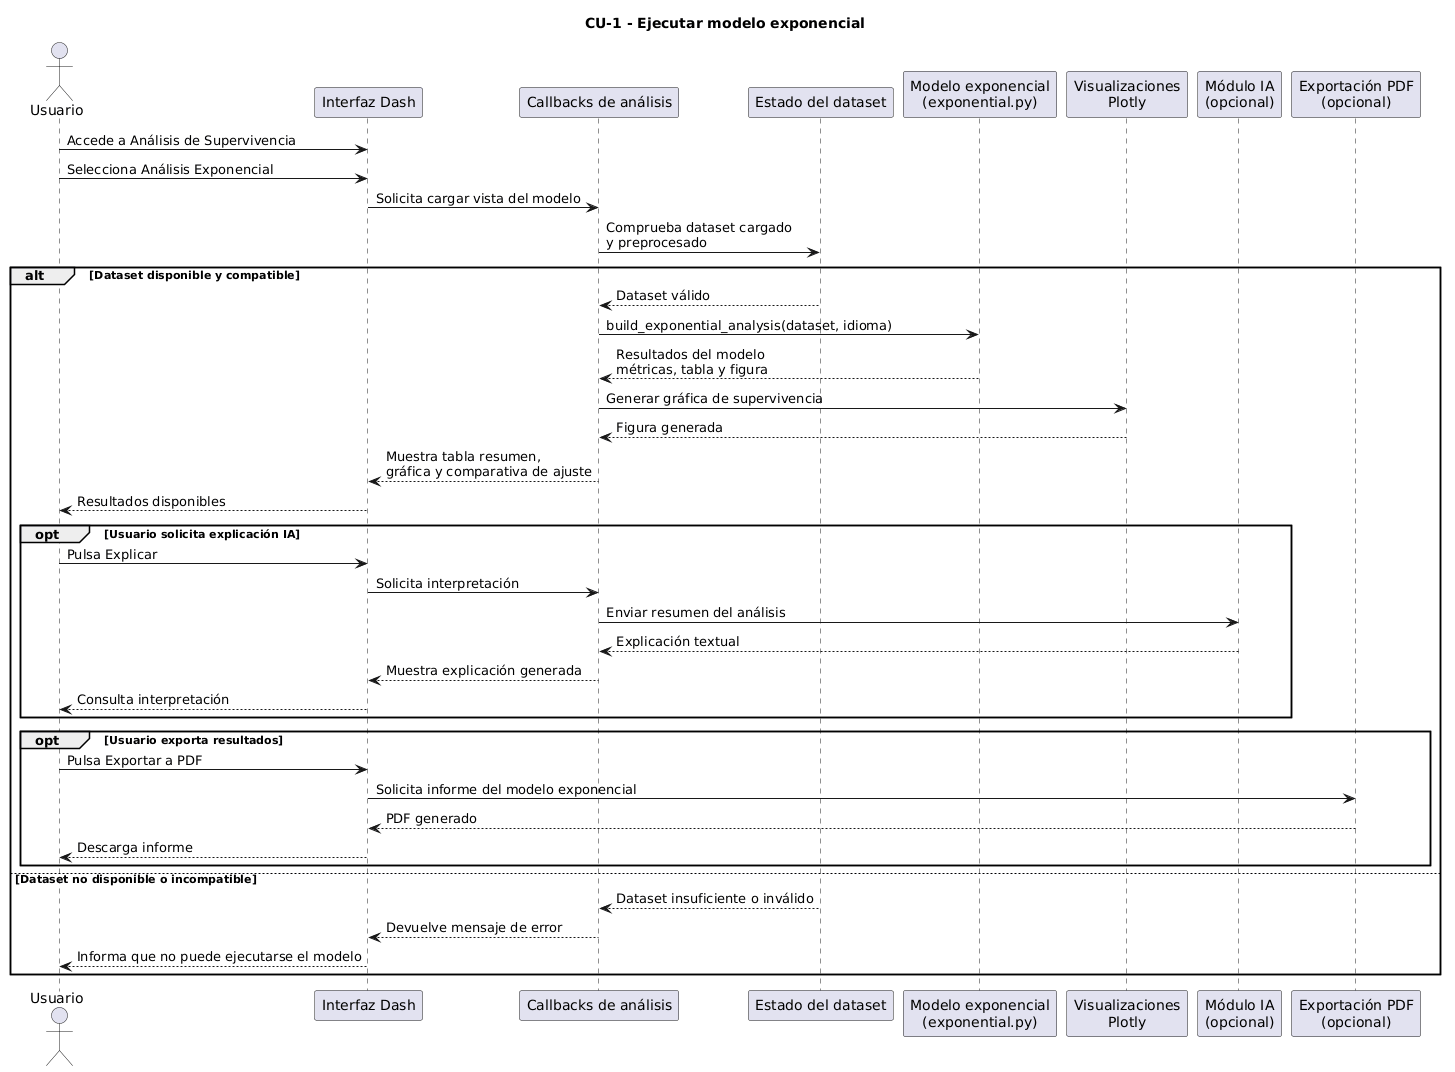
\includegraphics[width=\textwidth]{Imagenes/sec_cu1.png}
    \caption{Diagrama de secuencia del CU-1: EjecutarModeloExponencial}
    \label{fig:sec_cu1}
\end{figure}

\subsection{CU-2: EjecutarModeloWeibull}
\paragraph*{}
El diagrama del CU-2 representa el flujo interno necesario para ejecutar el modelo Weibull. La secuencia parte de la selección del análisis por parte del usuario, continúa con la validación del dataset y de los parámetros, y después delega el cálculo en el módulo \texttt{weibull.py}. Una vez obtenidos los resultados, se generan las visualizaciones correspondientes y se deja abierta la posibilidad de solicitar una explicación mediante IA o descargar el informe en PDF.

\begin{figure}[H]
    \centering
    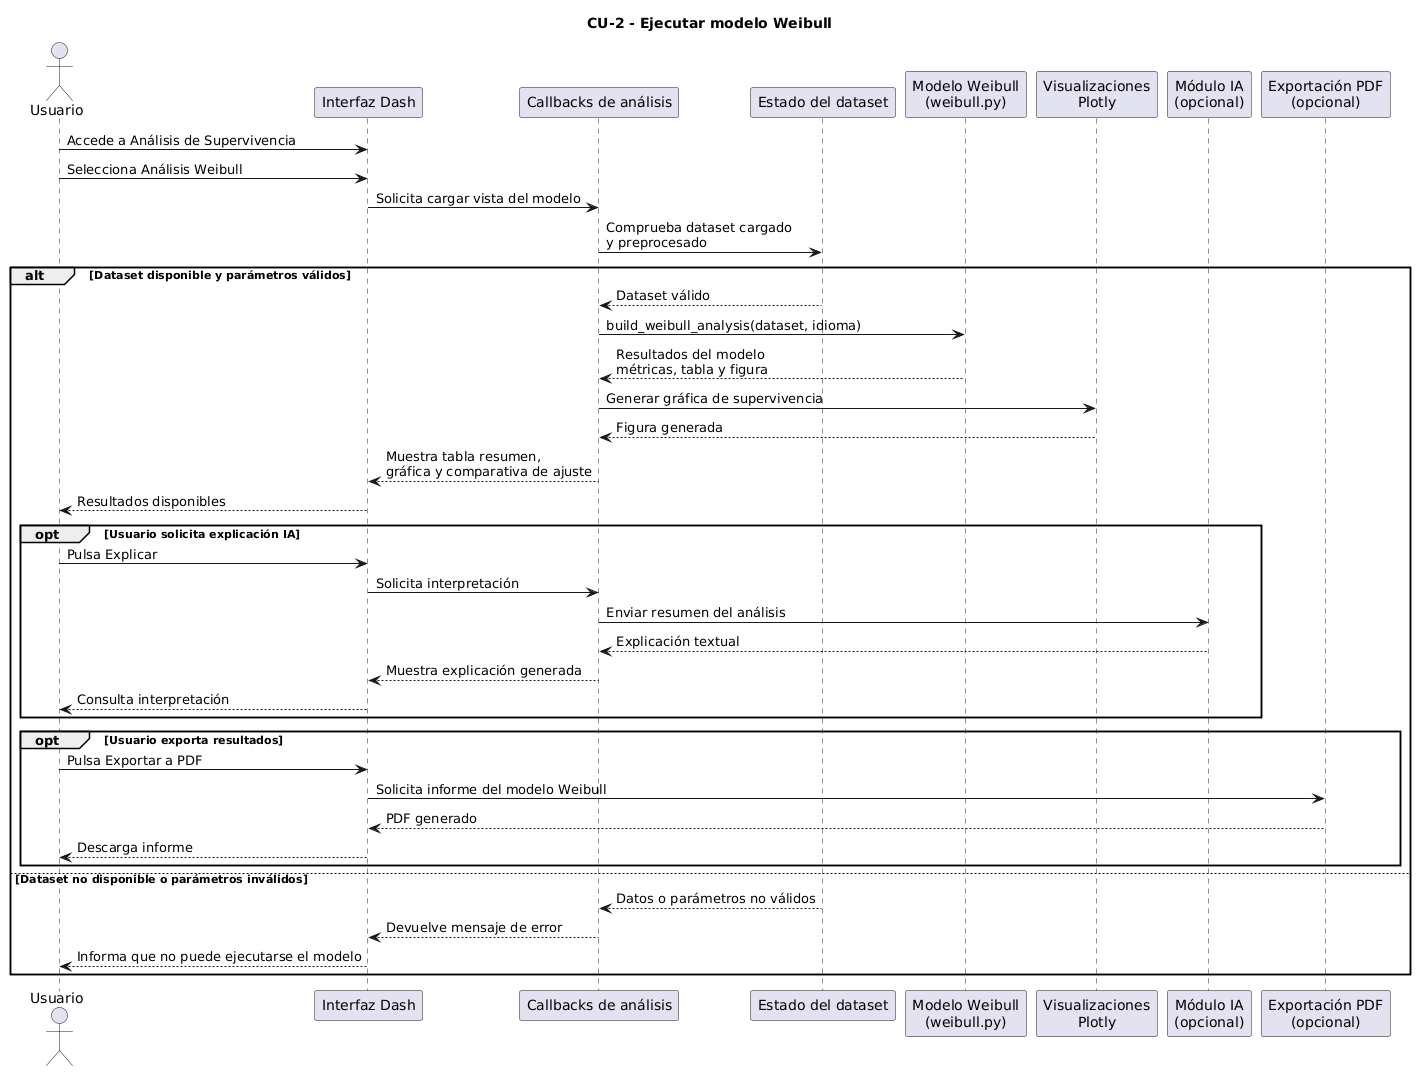
\includegraphics[width=\textwidth]{Imagenes/sec_cu2.png}
    \caption{Diagrama de secuencia del CU-2: EjecutarModeloWeibull}
    \label{fig:sec_cu2}
\end{figure}

\subsection{CU-3: EjecutarRandomSurvivalForest}
\paragraph*{}
El diagrama del CU-3 describe una interacción más completa, ya que Random Survival Forest no solo calcula resultados generales, sino que también permite simular perfiles personalizados. El sistema valida el dataset, ejecuta el análisis en \texttt{rsf.py}, genera curvas de supervivencia e importancia de variables y muestra los resultados en la interfaz. Después se contemplan acciones adicionales, como modificar los valores de un perfil, solicitar una interpretación automática o exportar el informe generado.

\begin{figure}[H]
    \centering
    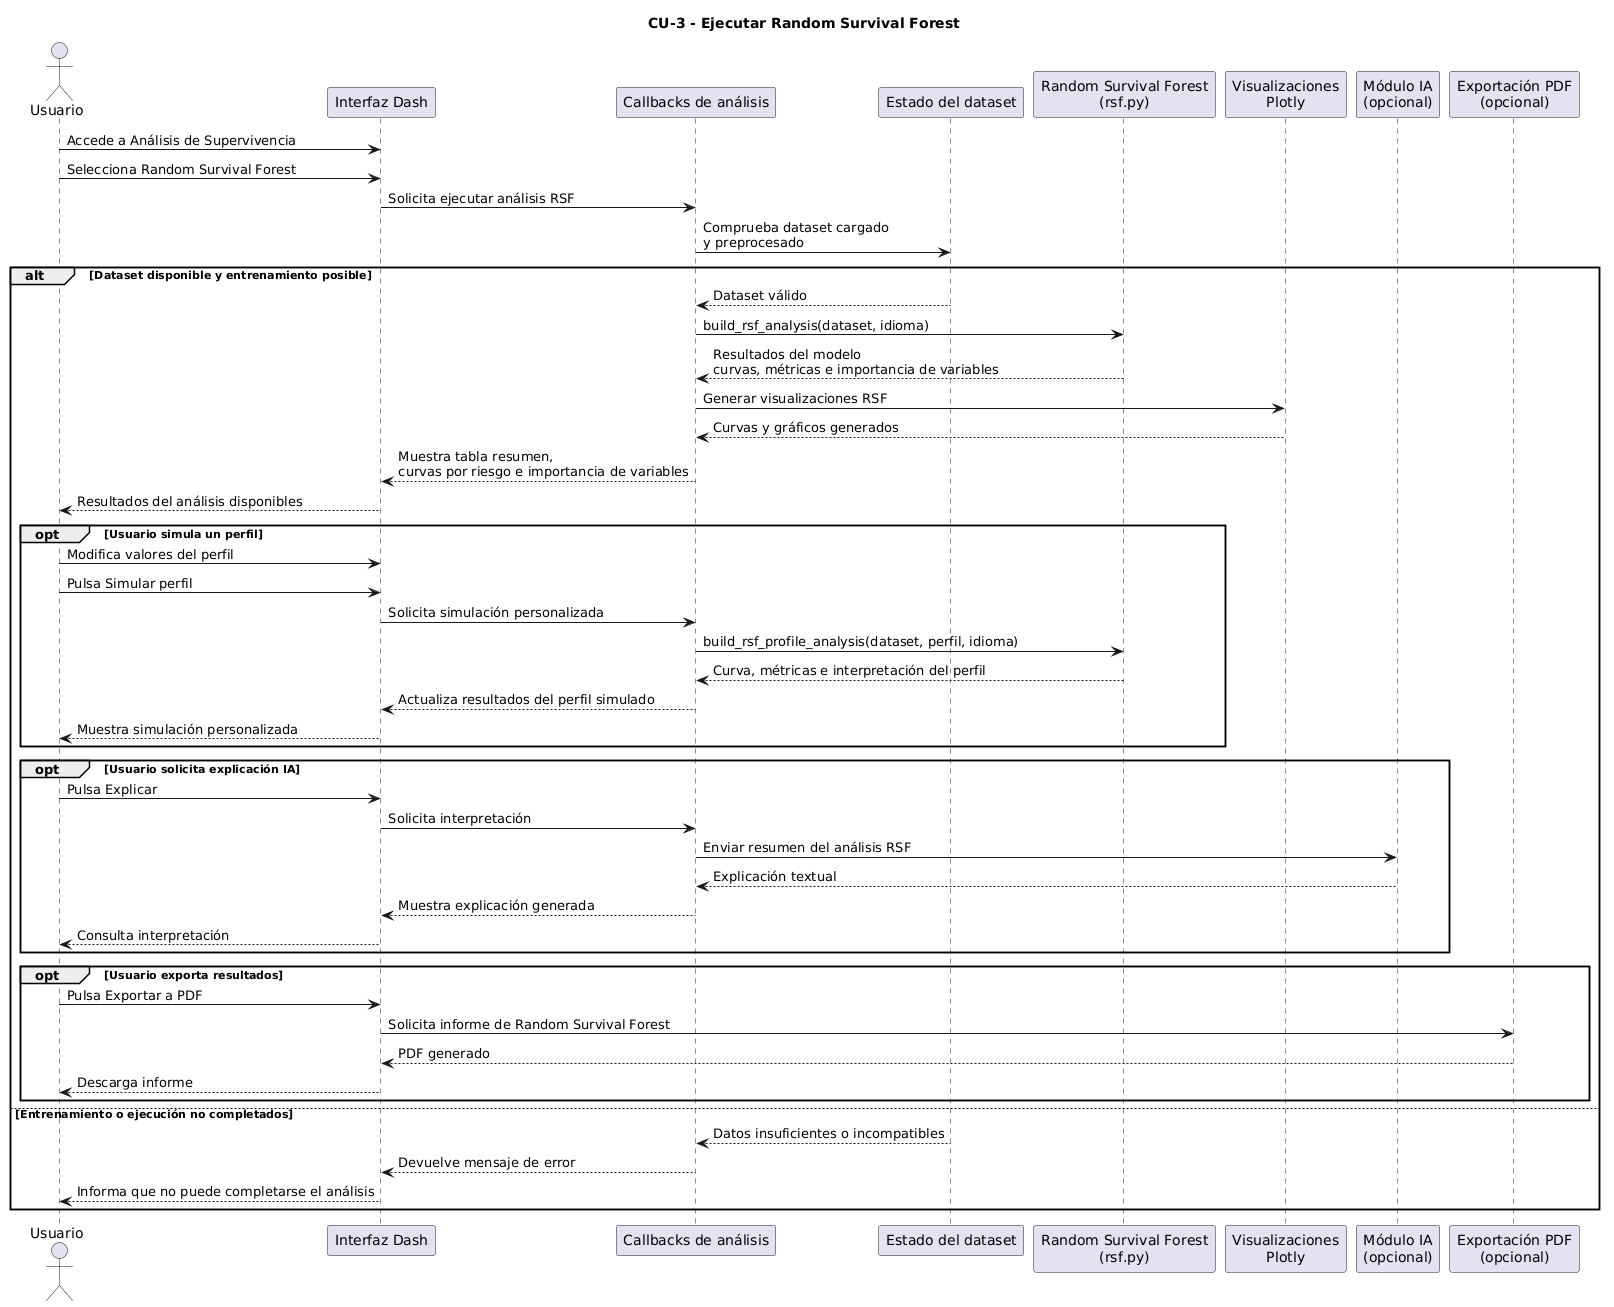
\includegraphics[width=\textwidth]{Imagenes/sec_cu3.png}
    \caption{Diagrama de secuencia del CU-3: EjecutarRandomSurvivalForest}
    \label{fig:sec_cu3}
\end{figure}

\subsection{CU-4: ConsultarComparacionDeTecnicas}
\paragraph*{}
El diagrama del CU-4 muestra cómo se construye la página de comparación de técnicas. Tras acceder desde el módulo de análisis de supervivencia, los callbacks comprueban que exista información disponible en sesión y solicitan la creación de la tabla comparativa, el gráfico de apoyo y el bloque explicativo automático. También se representan dos situaciones importantes: que no pueda generarse el gráfico comparativo o que falle la explicación mediante IA, en cuyo caso la página mantiene visible la información que sí se ha podido construir.

\begin{figure}[H]
    \centering
    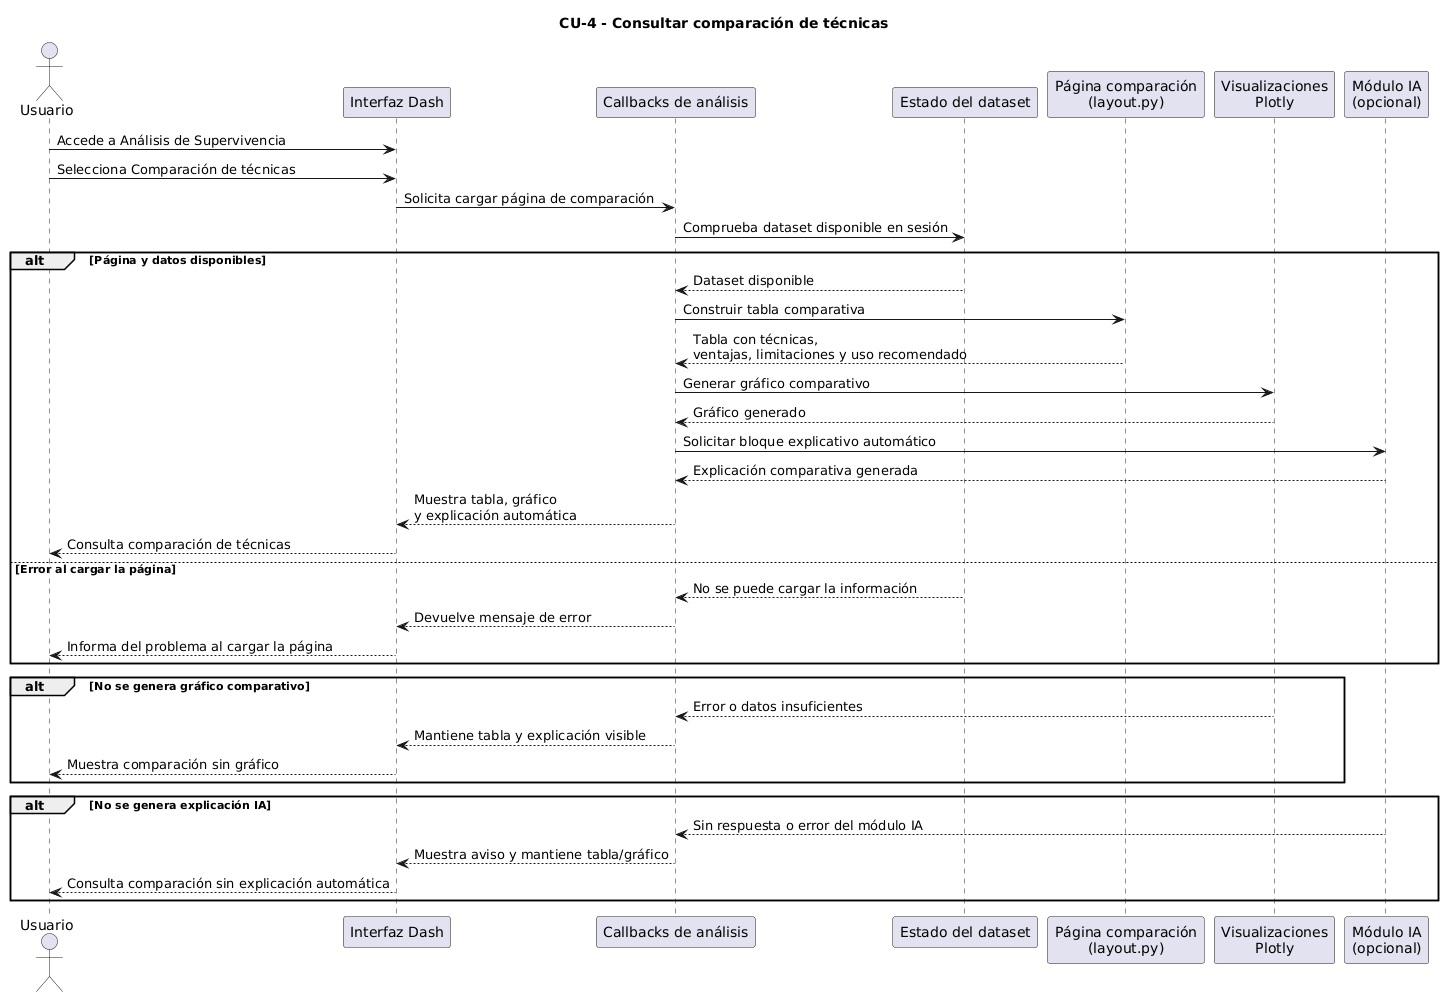
\includegraphics[width=\textwidth]{Imagenes/sec_cu4.png}
    \caption{Diagrama de secuencia del CU-4: ConsultarComparacionDeTecnicas}
    \label{fig:sec_cu4}
\end{figure}

\subsection{CU-5: ExportarInformesYResultados}
\paragraph*{}
El diagrama del CU-5 representa la generación de informes descargables. La secuencia comienza cuando el usuario abre el modal de exportación, introduce las opciones deseadas y solicita la descarga. A partir de ahí intervienen los callbacks de PDF, el estado del análisis y el exportador \texttt{SurvivalAnalysisPDFExporter}, que reúne resultados, convierte gráficas a imagen cuando es necesario, añade interpretaciones si se han seleccionado y guarda el documento en el sistema de archivos antes de devolverlo al usuario.

\begin{figure}[H]
    \centering
    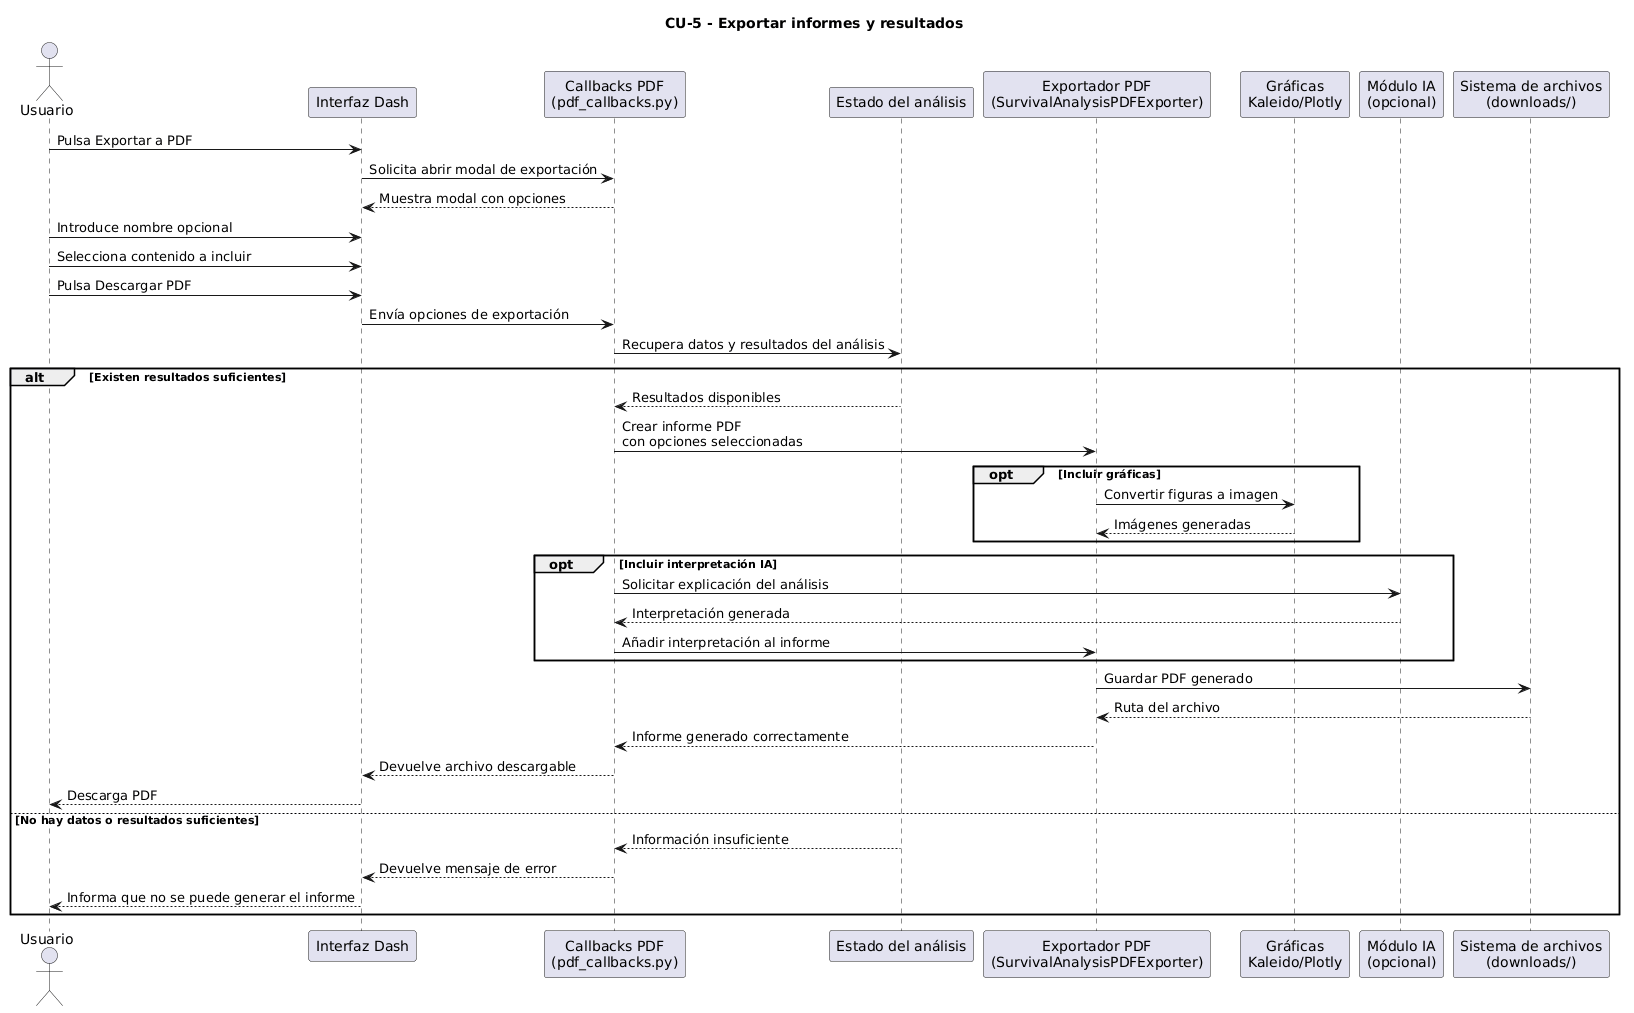
\includegraphics[width=\textwidth]{Imagenes/sec_cu5.png}
    \caption{Diagrama de secuencia del CU-5: ExportarInformesYResultados}
    \label{fig:sec_cu5}
\end{figure}

\subsection{CU-6: CambiarIdiomaInterfaz}
\paragraph*{}
El diagrama del CU-6 explica cómo se aplica el cambio de idioma en la interfaz. El usuario selecciona un idioma, el selector notifica el cambio a los callbacks de navegación y el sistema actualiza el estado del idioma activo. A continuación se recuperan las traducciones necesarias desde \texttt{translations.py} y se reconstruyen los componentes visibles del layout para actualizar menús, botones, títulos y mensajes sin modificar los datos cargados.

\begin{figure}[H]
    \centering
    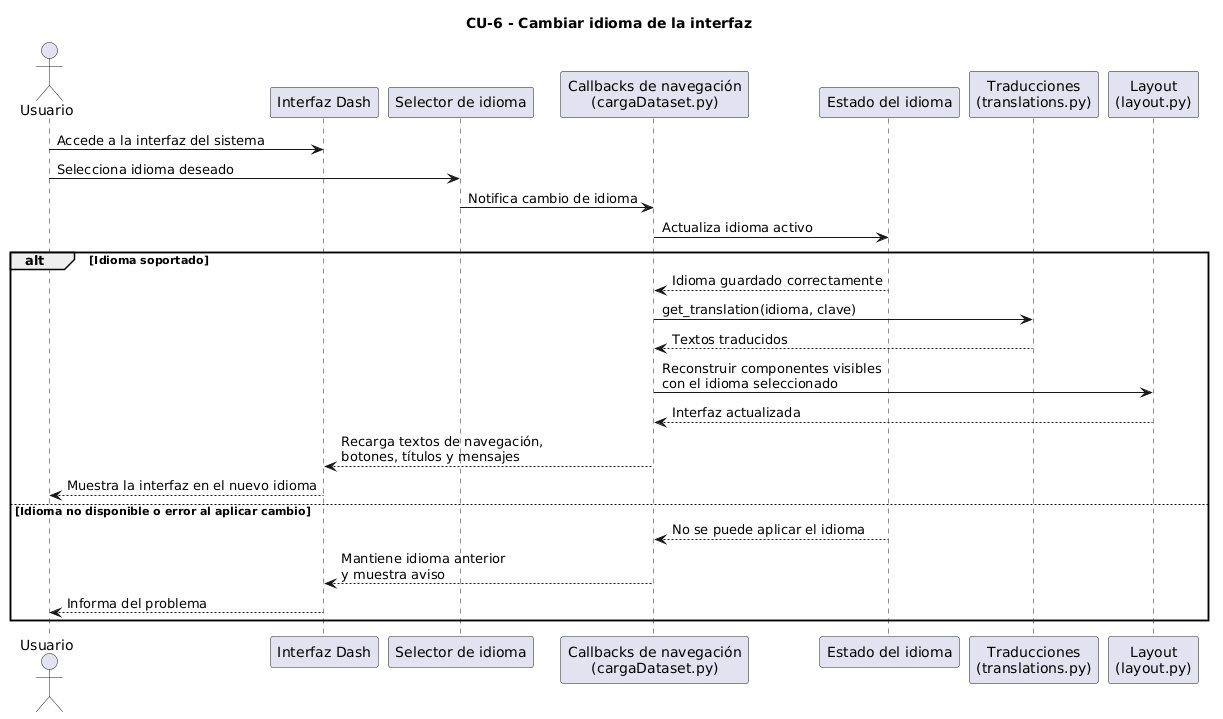
\includegraphics[width=\textwidth]{Imagenes/sec_cu6.png}
    \caption{Diagrama de secuencia del CU-6: CambiarIdiomaInterfaz}
    \label{fig:sec_cu6}
\end{figure}

\subsection{CU-7: AnalizarVariablesNoBinarias}
\paragraph*{}
El diagrama del CU-7 muestra el recorrido desde la carga del archivo CSV hasta el análisis de una variable no binaria. Primero se valida el formato del archivo y se ejecuta el preprocesamiento mediante \texttt{preprocesamiento.py}; después se guarda el dataset limpio y se recupera la variable seleccionada. Si la variable es compatible con el análisis, el sistema ejecuta el modelo correspondiente y genera tablas, métricas y visualizaciones. Si no lo es, se devuelve un mensaje de incompatibilidad al usuario.

\begin{figure}[H]
    \centering
    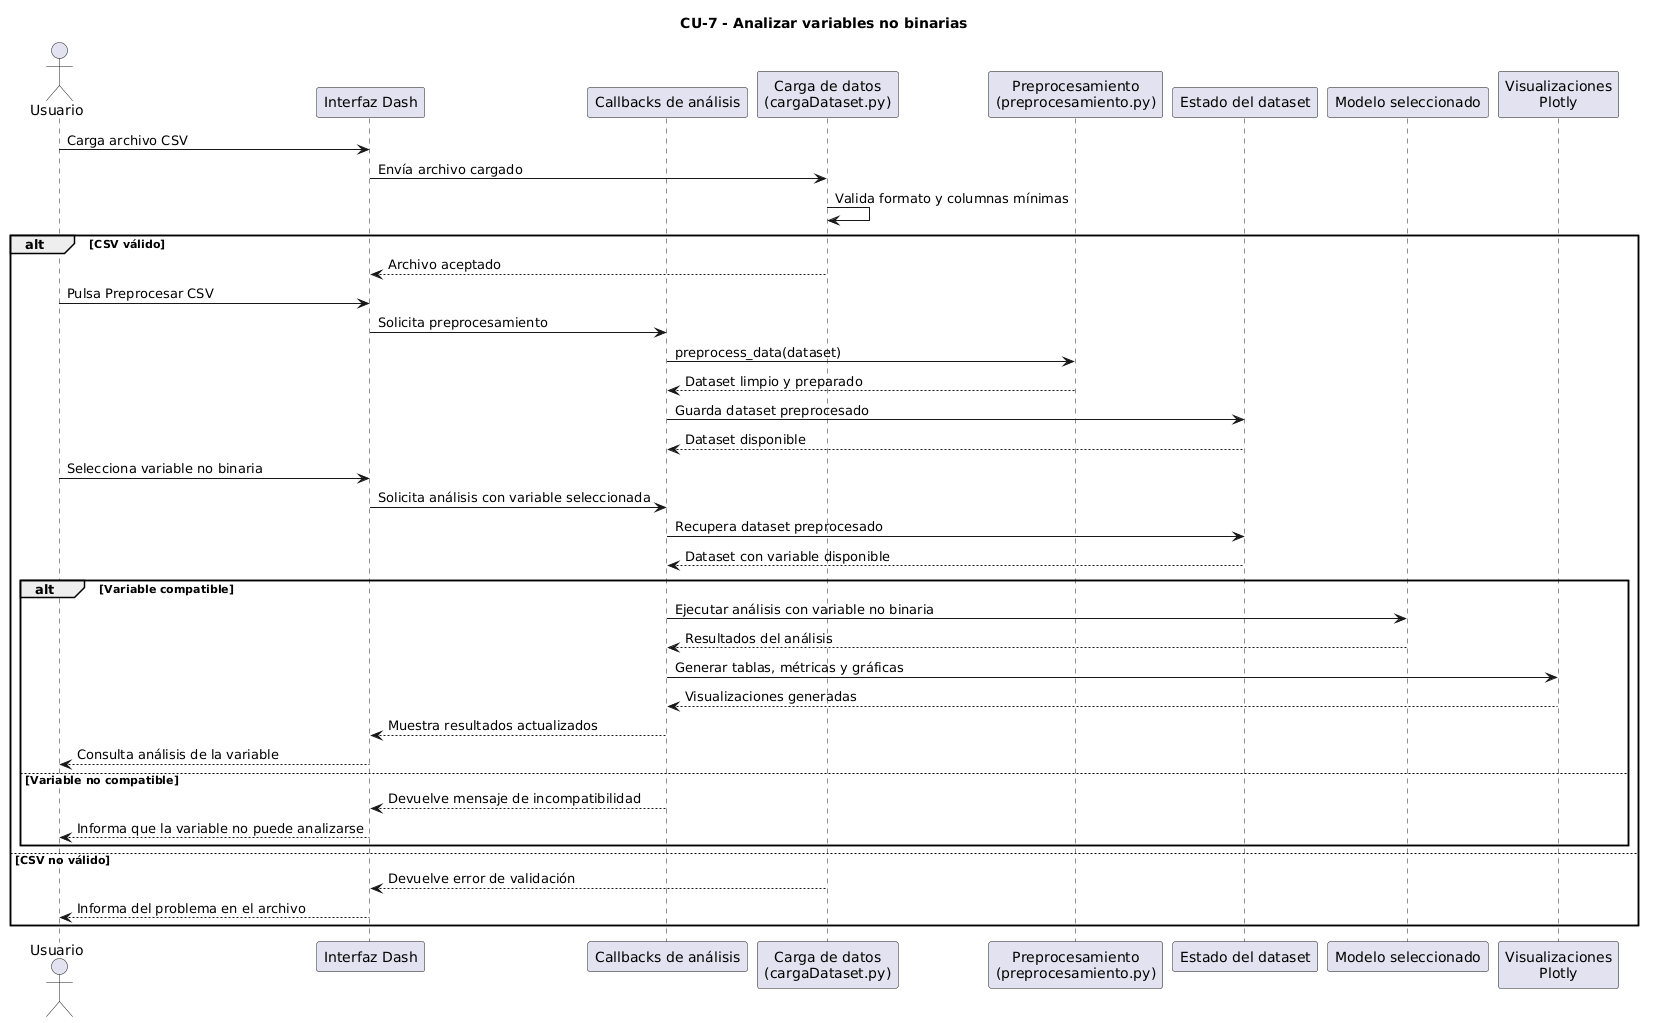
\includegraphics[width=\textwidth]{Imagenes/sec_cu7.png}
    \caption{Diagrama de secuencia del CU-7: AnalizarVariablesNoBinarias}
    \label{fig:sec_cu7}
\end{figure}

\subsection{CU-8: MejorarInterpretacionIA}
\paragraph*{}
El diagrama del CU-8 detalla el proceso de generación de interpretaciones mediante inteligencia artificial. La interfaz solicita una explicación, los callbacks recuperan los resultados disponibles y se construye un contexto textual con métricas, tablas y conclusiones relevantes. Ese contexto se envía al módulo \texttt{ollama\_AI.py}, que prepara la petición hacia el servidor local \texttt{llama-server} y el modelo Qwen. Finalmente, la respuesta se revisa, se formatea y se muestra al usuario, contemplando también los casos en los que no hay resultados previos o el módulo de IA no devuelve una respuesta válida.

\begin{figure}[H]
    \centering
    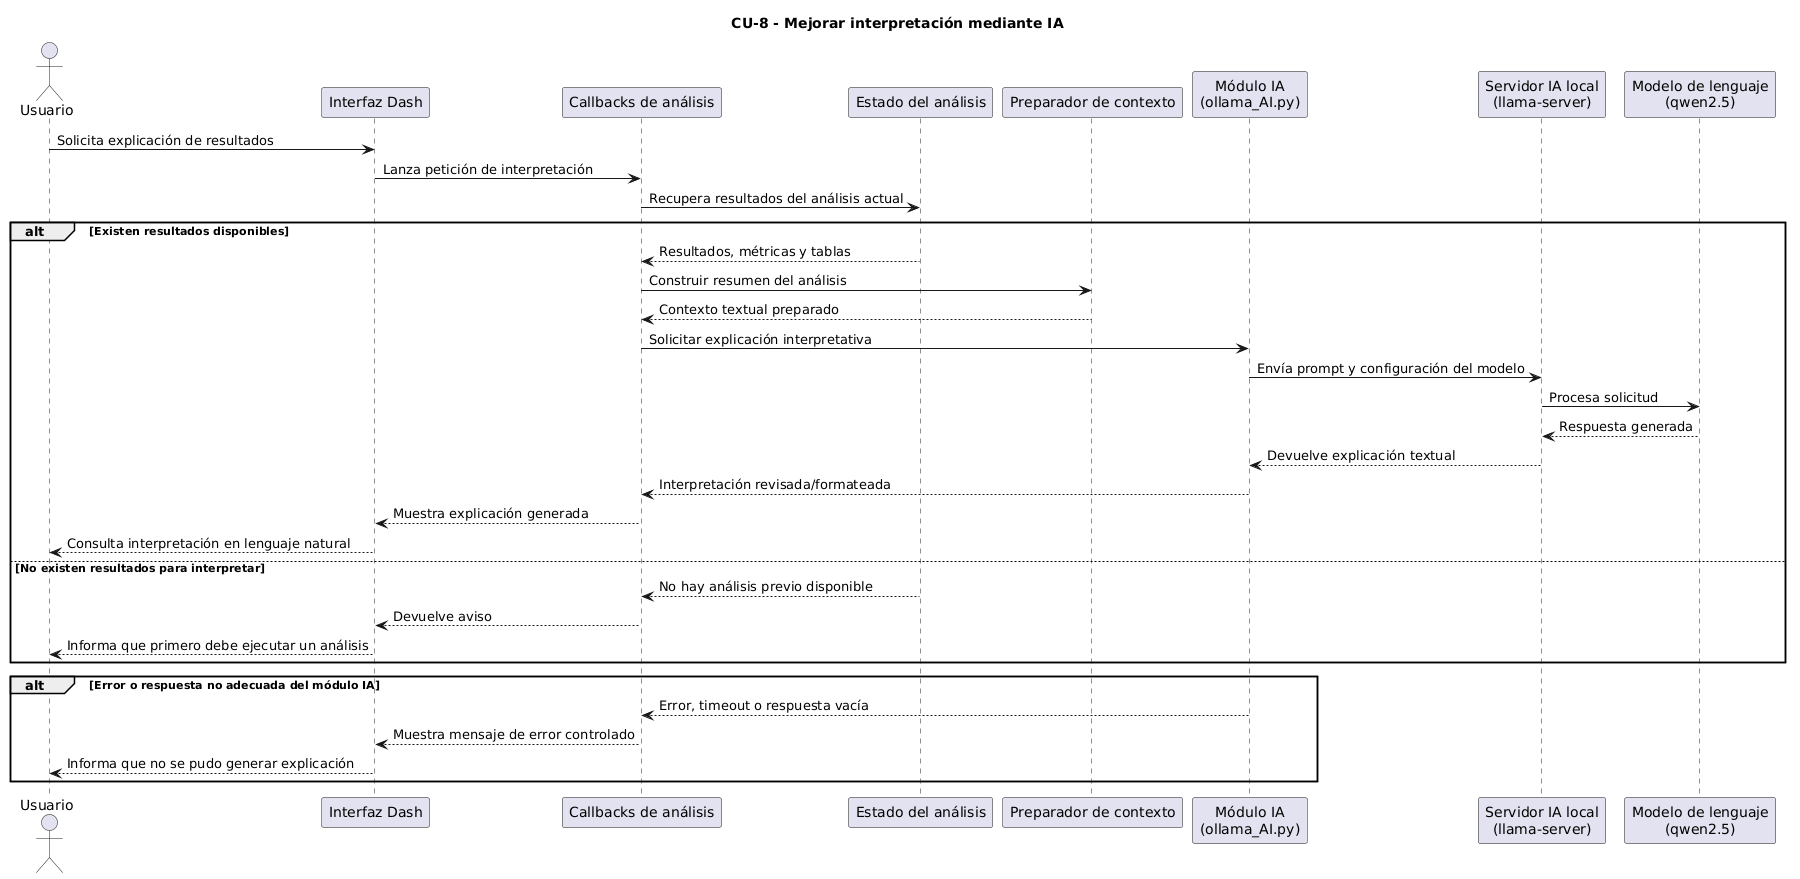
\includegraphics[width=\textwidth]{Imagenes/sec_cu8.png}
    \caption{Diagrama de secuencia del CU-8: MejorarInterpretacionIA}
    \label{fig:sec_cu8}
\end{figure}

\subsection{CU-9: AmpliarVisualizacionesCoxTestLogRank}
\paragraph*{}
El diagrama del CU-9 representa la generación de visualizaciones ampliadas para la regresión de Cox y el Test de Log-Rank. El sistema comprueba que existan datos y resultados previos, y después sigue un camino distinto según la visualización solicitada. Para Cox recupera los resultados de regresión y construye gráficos de hazard ratios; para Log-Rank obtiene la comparación entre grupos y genera curvas comparativas. En ambos casos, el módulo de visualizaciones prepara la figura con Plotly y devuelve la gráfica junto con los datos asociados.

\begin{figure}[H]
    \centering
    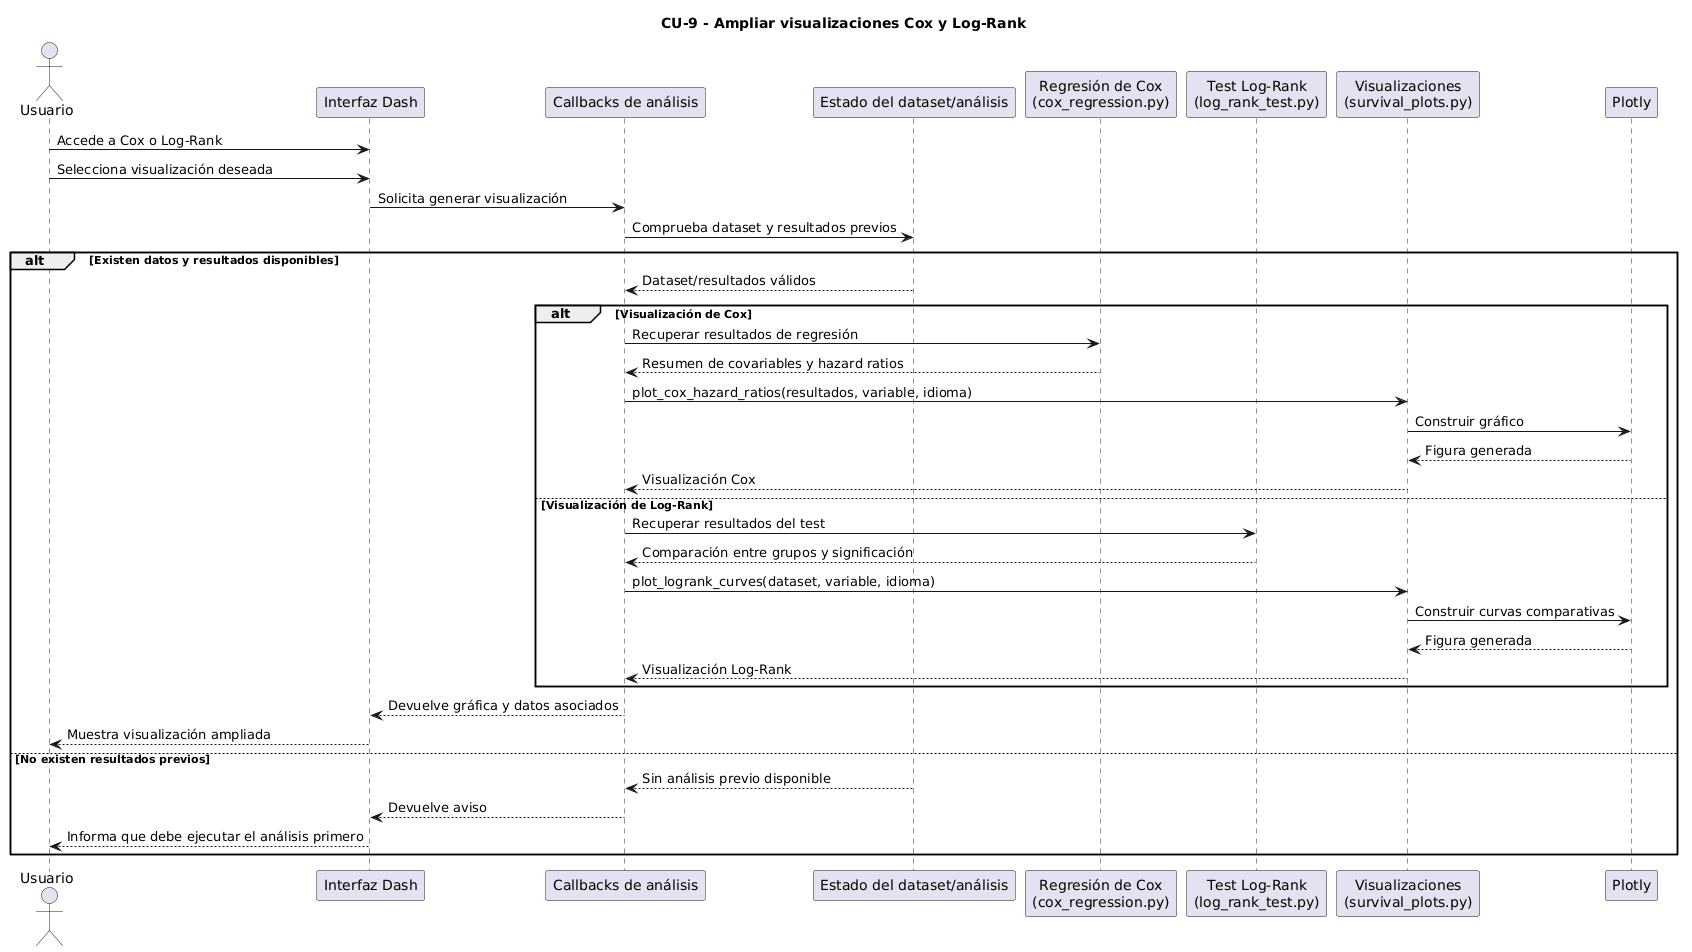
\includegraphics[width=\textwidth]{Imagenes/sec_cu9.png}
    \caption{Diagrama de secuencia del CU-9: AmpliarVisualizacionesCoxTestLogRank}
    \label{fig:sec_cu9}
\end{figure}
